\section{General results}
\label{general-results}

In this chapter, we study all the properties, equalities and inclusions from \cref{P:reg-star} for arbitrary $*$-language classes $\Lang$. We try to find necessary conditions such that the inclusions hold and also stay strict. And we demonstrate counter examples when they don't hold anymore or when inequalities become equalities.

We will also study some relations between the $\omega$-language classes constructed from $\Lang$ with the $\omega$-language classes constructed from $\Langreg$, i.e. the diagram as shown in \cref{regomega-diagram}. E.g. we will show that for some cases on $\Lang$, we have the equalities $\BC \lim \Lang \cap \lim \Langreg = \lim \Lang$ and $\BC \lim \Lang \cap \ext \Langreg = \ext \Lang$.

%S401: TODO

\

Let $\Lang$ be a $*$-language class. We start with some very basic results on language operators.

\subsection{Background}
We start with some generic properties, equalities and inclusions for the $\lim$ and $\ext$ operators.

\begin{lemma}
\label{gen:general}
Let $L,A,B \in \Lang$.
\begin{enumerate}
\item $\ext L = L \cdot \Sigma^\omega$
\item $\ext L = \lim(L \cdot \Sigma^*)$ %S303
\item $\ext L = \dlim(L \cdot \Sigma^*)$ %S303, S305.4
\item $- \lim(-L) = \dlim(L)$
\item $\dlim L \subseteq \lim L$
\item $\ext A \cup \ext B = \ext(A \cup B)$
\item $\dext A \cup \dext B \subseteq \dext(A \cup B)$ \\
There is no equality, i.e. `$\supseteq$` does not hold in general.
\item $\ext A \cap \ext B \supseteq \ext (A \cap B)$ \\
There is no equality, i.e. `$\subseteq$` does not hold in general.
\item $\lim A \cup \lim B = \lim(A \cup B)$ %S305.4
\item $\dlim A \cup \dlim B \subseteq \dlim(A \cup B)$ \\ %S305.4
There is no equality, i.e. `$\supseteq$` does not hold in general.
\item $\lim A \cap \lim B \supseteq \lim(A \cap B)$ \\
There is no equality, i.e. `$\subseteq$` does not hold in general.
\end{enumerate}
\begin{proof}
\begin{enumerate}
\item[1.-5.] They all follow directly from the definition.
\setcounter{enumi}{5}
\item
\begin{align*}
& \alpha \in \ext A \cup \ext B \\
\Leftrightarrow \ & \exists n \colon \alpha[0,n] \in A \ \vee \ \exists n \colon \alpha[0,n] \in B \\
\Leftrightarrow \ & \exists n \colon \alpha[0,n] \in A \cup B \\
\Leftrightarrow \ & \alpha \in \ext A \cup B
\end{align*}
\item
\begin{align*}
& \alpha \in \dext A \cup \dext B \\
\Leftrightarrow \ & \forall n \colon \alpha[0,n] \in A \ \vee \ 
\forall n \colon \alpha[0,n] \in B \\
\Rightarrow \ & \forall n \colon \alpha[0,n] \in A \cup B \\
\Leftrightarrow \ & \alpha \in \dext (A \cup B)
\end{align*}

Consider the languages $A := (aa)^*$, $B := (aa)^*a$. Then,
\[ \dext(A \cup B) = \dext(a^*) = a^\omega \ne \emptyset = \emptyset \cup \emptyset = \dext A \cup \dext B . \]
\item That is just (\addtocounter{enumi}{-1}\arabic{enumi}\addtocounter{enumi}{+1}) negated.
\item %S305.4
\begin{align*}
& \alpha \in \lim A \cup \lim B \\
\Leftrightarrow \ & \existsinf n \colon \alpha[0,n] \in A \ \vee \ \existsinf n \colon \alpha[0,n] \in B \\
\Leftrightarrow \ & \existsinf n \colon \alpha[0,n] \in A \cup B \\
\Leftrightarrow \ & \alpha \in \lim A \cup B
\end{align*}

\item %S305.4
\begin{align*}
& \alpha \in \dlim A \cup \dlim B \\
\Leftrightarrow \ & \exists N \colon \forall n \ge N \colon \alpha[0,n] \in A \ \vee \ 
\exists N \colon \forall n \ge N \colon \alpha[0,n] \in B \\
\Rightarrow \ & \exists N \colon \forall n \ge N \colon \alpha[0,n] \in A \cup B \\
\Leftrightarrow \ & \alpha \in \dlim (A \cup B)
\end{align*}

Consider the languages $A := (aa)^*$, $B := (aa)^*a$. Then,
\[ \dlim(A \cup B) = \dlim(a^*) = a^\omega \ne \emptyset = \emptyset \cup \emptyset = \dlim A \cup \dlim B . \]

\item That is just (\addtocounter{enumi}{-1}\arabic{enumi}\addtocounter{enumi}{+1}) negated.
\end{enumerate}
\end{proof}
\end{lemma}

For $\omega$ automata, we already know that non-determinism can be more powerful than determinism (see \cref{reg-omega-lang}): The class of non-deterministic Büchi automata can accept clearly more languages than the class of deterministic Büchi automata. E.g. $L_\omega := (a+b)^* b^\omega \in \LangOreg$ cannot be recognized by deterministic Büchi automata, i.e. $L_\omega \not\in \lim \Langreg$.

Luckily, for E- and A-acceptance, this is not the case as we see below. This matches the intuition that E/A-acceptance doesn't really tell something about infinitary properties of words but Büchi/Muller does. And when talking about finite words, we already know that non-deterministic and deterministic automata are equally powerful (see \cref{intro:reglang}).

%307.12
\begin{lemma}
\label{gen:e-determinism}
The $\omega$-language-class accepted by deterministic E-automata is equal to non-deterministic E-automata. I.e., for every non-deterministic E-automaton, we can construct an equivalent deterministic E-automaton. The same holds for A-automata.
\begin{proof} Let $\A^N$ be any non-deterministic automaton and $\A^D$ an ($*$-)equivalent deterministic automaton. Then:
\begin{align*}
& \alpha \in L^{\omega}_E(\A^N) \\
\Leftrightarrow \ & \exists n \colon \alpha[0,n] \in L(\A^N) \\
\Leftrightarrow \ & \exists n \colon \alpha[0,n] \in L(\A^D) \\
\Leftrightarrow \ & \alpha \in L^{\omega}_E(\A^D)
\end{align*}
$\A^N$ can be interpreted as an arbitrary E-automata and we have shown that we get an equivalent deterministic E-automata.

For A-automata, the proof is analogous.
\end{proof}
\end{lemma}

\

%S302.1:
We are interested in relations like $\BC \ext \Lang \overset{?}{\subsetneqq} \BC \lim \Lang$ or $\ext \Lang \overset{?}{\subsetneqq} \lim \Lang$. With $\Lang = \Set{\Set{a}}$, we realize that even $\ext \Lang \subseteq \lim \Lang$ is not true in general ($\ext \Set{\Set{a}} = \Set{a \Sigma^\omega} \neq \emptyset = \lim \Set{\Set{a}}$). In \cref{gen:non-suffix-sens}, we see a sufficient condition for this property, though.

We want to study all the properties we have shown for $\Langreg$ in \cref{P:reg-star}.

\

We will formulate some properties of interest in a general form for a $*$-language class $\Lang$ which all hold for $\Langreg$. We get some general results based on these properties later in this chapter. %\ref{general-results}.

%S303.E3, S218, R101
Let $L,A,B \in \Lang$. Then there are the following properties on $\Lang$:
\begin{enumerate}
\item[1.] \defword{Closure under suffix-independence}: $L \cdot \Sigma^* \in \Lang$

We call $L$ \defword{suffix-independent} iff $L = L \Sigma^*$. However, we are mostly interested in the language class closure.

For language classes defined via subsets of regular expressions, we often can directly check wether we have this closure property. It means that we can add "$\cdot\Sigma^*$" at the end of a regular expression and we will stay in the same language class. E.g. for the starfree languages (as defined in \cref{lang:starfree}), this is the case.

However, this closure is a very strong property as we will see later (e.g. in \cref{gen:R-suffix-indep->single-state-loops}). An example of a simple language class which is not closed under suffix-independence is given in \cref{gen:example:non-suffixindep-closure}.

\item[2a.] \defword{Closure under union}: $A \cup B \in \Lang$
\item[2b.] \defword{Closure under intersection}: $A \cap B \in \Lang$
\item[3.] \defword{Closure under complementation/negation}: $- L \in \Lang$

\item[4.]
\defword{Closure under change of final states}:
Let $\A_L = (Q,\Sigma,q_0,\delta,F_L)$ be the minimal deterministic automaton for $L$, i.e. with $L^*(\A_L) = L$. Then, for all $F' \subseteq Q$, we have $L^*((Q,\Sigma,q_0,\delta,F')) \in \Lang$.

%S303.1:
In some proofs, e.g. in \cref{gen:staiger-wagner} or \cref{gen:kleene-star}, we have an automaton based on some language of the language class and we do some modifications on it, e.g. we modify the acceptance component.

For $\Langreg$, this closure property holds obviously. For other language classes, it is much less clear. However, we will see a whole class of language classes where this closure property holds, namely the congruence-based language classes as defined in \cref{gen:R}. Also, when we have some structure property on the transition graph independent from the final state set for all languages in a class, in many cases it holds that changing the final states keeps the structure property and thus we have the closure under change of final states. An example where we have this is the class of starfree languages (defined in \cref{lang:starfree}) where each minimal deterministic automata is counter-free (see \cref{lang:starfree:closurefinalstates}).

%S303.1.a:
Note that we cannot just take any automaton. For $\Lang^*(\mathtext{starfree})$ (see \cref{lang:starfree}) and the automaton below, it does not hold:

  \begin{tikzpicture}[%
    >=stealth,
	shorten >=1pt,
	node distance=2cm,
%    on grid,
    auto,
%    state/.append style={minimum size=2em},
%    thick
  ]
    \node[state] (S)              {};
    \node[state,double] (A) [right of=S] {$A$};
    \node[state] (B) [below of=S] {$B$};
    \node[state] (C) [right of=B] {};

    \path[->] (S) +(-1,0) edge (S)
              (S)         edge              node {$a$} (A)
              (S)         edge              node {$b$} (B)
              (B)         edge  [bend left]            node {$b$} (C)
              (C)         edge  [bend left]            node {$b$} (B)
              ;
  \end{tikzpicture}
  
This is a deterministic automaton for the language $\Set{a} \in \Lang^*(\mathtext{starfree})$. If you make $B$ also a final state, we get the language $a + b(bb)^* \not\in \Lang^*(\mathtext{starfree})$.

\item[5.] \defword{Closure under alphabet permutation}: For all permutations $\sigma : \Sigma \rightarrow \Sigma$, we have $L_\sigma := \Set{\sigma(w)}{w \in L} \in \Lang$. ($\sigma$ on words is defined canonically.)

If $L = L_\sigma$ for all permutations $\sigma$, we call $L$ \defword{alphabet permutation invariant}.

\end{enumerate}

\subsection{Classification for arbitrary language classes}
\label{gen:section:classification}

We will first study $\ext \Lang \subseteq \lim \Lang$ inclusions. We have the very simple result:
%\subsection{non suffix sensitive}
% S303, S101a:
\begin{lemma}
\label{gen:non-suffix-sens}
If $\Lang$ is closed under suffix-independence, then
\[ \ext \Lang \subseteq \lim \Lang \cap \dlim \Lang . \]
\begin{proof}
For $L \in \Lang$, we have $\ext L = L \Sigma^\omega = \lim (L \Sigma^*) = \dlim (L \Sigma^*)$.
\end{proof}
\end{lemma}

However, there is no equivalence. Closure under suffix-independence is a very strong property as can be seen in \cref{gen:R-suffix-indep->single-state-loops}.
\begin{example}
\label{gen:example:non-suffixindep-closure}
There is a $*$-language class $\Lang$ with $\ext \Lang \subseteq \lim \Lang$ which is not closed under suffix-independence.
\begin{proof}
Consider the transition graph $\A = (Q,\Sigma,q_0,\delta)$:
\[
  \begin{tikzpicture}[%
    >=stealth,
	shorten >=1pt,
	node distance=2cm,
    auto,
  ]
    \node[state] (1)              {$1$};
    \node[state] (2) [right of=1] {$2$};

    \path[->]
    (1) +(-1.5,0) edge (1)
    (1) edge [bend left] node {$\Sigma$} (2)
    (2) edge [bend left] node {$\Sigma$} (1)
    ;
  \end{tikzpicture}
\]
Let $\Lang := \Set{L^*(\A(F))}{F \subseteq Q}$. I.e. $L_2 := \Sigma(\Sigma\Sigma)^* \in \Lang$ (all words ending in state $2$). Then, $L_2 \Sigma^* = \Sigma^+ \not\in \Lang$. I.e. $\Lang$ is not closed under suffix-independence. However, we have
\[ \ext \Lang = \dext \Lang = \Set{\emptyset, \Sigma^\omega} = \lim \Lang = \dlim \Lang . \]
\end{proof}
\end{example}

%\subsection{$\BC \ext \subseteq \BC \lim$}
%S302:
\begin{lemma}
\label{gen:S302a} If we have $\ext \Lang \subseteq \lim \Lang$, then we also have
\[ \BC \ext \Lang \subseteq \BC \lim \Lang . \]
\begin{proof}
From $\ext \Lang \subseteq \lim \Lang$, it directly follows $\Set{-\ext L}{L \in \Lang} \subseteq \Set{-\lim L}{L \in \Lang}$. Thus, it also follows the claimed inequality.
\end{proof}
\end{lemma}

%\subsection{$\dext \subset \dlim$}
%S302:
\begin{lemma}
\label{gen:DExtInDLim}
If we have $\ext \Lang \subseteq \lim \Lang$ and let $\Lang$ be closed under negation. Then we have
\[ \dext \Lang \subseteq \dlim \Lang . \]
\begin{proof}
Let $L \in \Lang$. Then $ \dext L = - \ext (-L) $. Because of the negation closure, we also have $-L \in \Lang$ and $\ext(-L) \in \ext \Lang$.

Thus $\ext(-L) \in \lim \Lang$. Thus, $\dext(L) = -\ext(-L) \in \Set{-\lim A}{A \in \Lang} = \Set{\dlim A}{-A \in \Lang}$. Because of the negation closure, we have
\[ \Set{\dlim A}{-A \in \Lang} = \Set{\dlim A}{A \in \Lang} = \dlim \Lang . \]
Thus,
\[ \dext L \in \dlim \Lang . \]
\end{proof}
\end{lemma}

Note that we needed the closure under negation in the proof. This is in contrast to \cref{gen:S302a}, where it directly follows. We have to be careful about the inequality
\[ \neg\ext \Lang := \Set{-\ext L}{L \in \Lang} \neq \dext \Lang \]
(in general, if $\Lang$ is not closed under negation).

Analogously:

\begin{lemma}
\label{gen:DExtInLim}
If we have $\ext \Lang \subseteq \dlim \Lang$ and let $\Lang$ be closed under negation. Then we have
\[ \dext \Lang \subseteq \lim \Lang . \]
\begin{proof}
Let $L \in \Lang$. Then $ \dext L = - \ext (-L) $. Because of the negation closure, we also have $-L \in \Lang$ and $\ext(-L) \in \ext \Lang$.

Thus $\ext(-L) \in \dlim \Lang$. Thus, $\dext(L) = -\ext(-L) \in \Set{-\dlim A}{A \in \Lang} = \Set{\lim A}{-A \in \Lang}$. Because of the negation closure, we have
\[ \Set{\lim A}{-A \in \Lang} = \Set{\lim A}{A \in \Lang} = \lim \Lang . \]
Thus,
\[ \dext L \in \lim \Lang . \]
\end{proof}
\end{lemma}

Summarized:

\begin{lemma}
\label{gen:extInLim}
Let $\Lang$ be closed under suffix-independence and negation. Then we have
\[ \ext \cup \dext \Lang \subseteq \lim \cap \dlim \Lang . \]
\begin{proof}
This is lemma \ref{gen:non-suffix-sens}, \ref{gen:DExtInDLim} and \ref{gen:DExtInLim}.
\end{proof}
\end{lemma}

Note that we don't always have $\ext \Lang \subseteq \lim \Lang$. For one example with some strict properties see \cref{gen:example:R-extNotInLim}. Another example with separates $\ext \Lang$ and $\lim \Lang$ even more:
\begin{example}
\label{gen:example:ext<->lim}
There is a $*$-language class $\Lang$, closed under negation, union, intersection and change of final states such that
\[ \ext \Lang \not\subseteq \lim \Lang , \ \ \ \ext \Lang \not\supseteq \lim \Lang . \]
\begin{proof}
Let $\Sigma = \Set{a,b}$. Look at the transition graph $\A = (Q,\Sigma,q_0,\delta)$:
\[
  \begin{tikzpicture}[%
    >=stealth,
	shorten >=1pt,
	node distance=2cm,
    auto,
  ]
    \node[state] (1)              {$1$};
    \node[state] (2) [right of=1] {$2$};
    \node[state] (3) [below of=1] {$3$};

    \path[->]
    (1) +(-1.5,0) edge (1)
    (1) edge [bend left] node {$a$} (2)
    (2) edge node {$a,b$} (1)
    (1) edge node {$b$} (3)
    (3) edge [bend left] node {$a,b$} (1)
    ;
  \end{tikzpicture}
\]
Then define $\Lang := \Set{L^*(\A(F))}{F \subseteq Q}$. $\A$ is deterministic, thus $\Lang$ is closed under negation, union, intersection and change of final states.

Let $L_2 := a (\Sigma (b \Sigma)^* a)^* \in \Lang$ (all words ending in state $2$). Then $\ext L_2 = a\Sigma^\omega \not\in \BC \lim \Lang$.

Also, $\lim L_2 = \Set{\alpha \in \Sigma^\omega}{\text{$\alpha$ visits state $2$ infinitely often}} \not\in \BC \ext \Lang$.

In this example, we can see that
\[ \BC \ext \Lang \cup \BC \lim \Lang \subsetneqq \BC (\ext \cup \lim) \Lang . \]
$\omega$-languages from $\BC (\ext \cup \lim) \Lang$ express which states will be visited, which will not be visited and which will be visited infinitely often and which not.
\end{proof}
\end{example}

We need the \emph{negation closure} for the natural expected inclusion of the dual operators in their boolean closures.

\begin{lemma}
\label{gen:opinBCop}
Let $\Lang$ be closed under negation. Then
\[ \ext \cup \dext \Lang \subseteq \BC \ext \Lang , \]
\[ \lim \cup \dlim \Lang \subseteq \BC \lim \Lang . \]
\begin{proof}
Because of the negation closure, we have
\[ \BC \ext \Lang \supseteq \Set{-\ext A}{A \in \Lang} = \Set{\dext A}{-A \in \Lang} = \dext \Lang , \]
\[ \BC \lim \Lang \supseteq \Set{-\lim A}{A \in \Lang} = \Set{\dlim A}{-A \in \Lang} = \dlim \Lang . \]
\end{proof}
\end{lemma}

%\subsection{union, intersection}
%S303:
%\begin{lemma}
%\begin{itemize}
%\item
%$\Lang$ closed under union $\Rightarrow \bigcup \ext \Lang \subseteq \ext \Lang$.
%\item
%$\Lang$ closed under intersection $\Rightarrow \bigcap \ext \Lang \subseteq \ext \Lang$.
%\end{itemize}
%\begin{proof}
%Let $A,B \in \Lang$. Then we have $\ext(A\cup B) = \ext(A) \cup \ext(B)$.
% and $\ext(A\cap B) = \ext(A) \cap \ext(B)$. % no, we don't have that...
%\end{proof}
%\end{lemma}

We present some common examples which would separate $\ext\cup\dext \Lang$ from $\BC \ext \Lang$ and similarly $\lim\cup\dlim \Lang$ from $\BC \lim \Lang$.

\begin{example}
\label{gen:example:extBCextSeparate}
Let $\Set{a,b,c} \subseteq \Sigma$. Define $L_a := \Sigma^*a$, $L_b := \Sigma^*b$. Let $L_a,L_b \in \Lang$. Let $\Lang$ be closed under negation. Then
\[ \ext \cup \dext \Lang \subsetneqq \BC \ext \Lang , \]
\[ \lim \cup \dlim \Lang \subsetneqq \BC \lim \Lang . \]
\begin{proof}
The inclusion follows from lemma \ref{gen:opinBCop}.

$\tilde L_1 := \ext(L_a) \cap -\ext(L_b)$. Then $\tilde L_1 \not\in \ext \cup \dext \Lang$ but $\tilde L_1 \in \BC \ext \Lang$. (\Cref{P:reg-star})

$\tilde L_2 := \lim(L_a) \cap -\lim(L_b)$. Then $\tilde L_2 \not\in \lim \cup \dlim \Lang$ but $\tilde L_2 \in \BC \lim \Lang$. (\Cref{P:reg-star})
\end{proof}
\end{example}

This example can be generalized a bit. We first introduce $M$-invariance on a language for $M\subseteq\Sigma$.

\begin{mydef}
A language $L \subseteq \Sigma^*$ is called \defword{$M$-invariant} for $M \subseteq\Sigma$ iff for all $w_1,w_2 \in \Sigma^*$, $a \in M$,
\[ w_1 a w_2 \in L \ \ \ \Rightarrow \ \ \  w_1 M^* w_2 \subseteq L . \]
%
%There is always exactly one \defword{maximum invariant alphabet set $M_{max} \subseteq \Sigma$ of $L$} such that $L$ is $M_{max}$-invariant. Then call $\Sigma-M_{max}$ the \defword{non-invariant alphabet set of $L$}.
%
A language $L \subseteq \Sigma^*$ is called $M$-\defword{relevant} iff $L$ is not $M$-invariant and $\Sigma^* a \Sigma^* \cap L \ne \emptyset$ for every $a \in M$.
\end{mydef}

\begin{mydef}
For $L \subseteq \Sigma^* \cup \Sigma^\omega$, $M \subseteq \Sigma$, define
\[ L|_M := L \cap (M^* \cup M^\omega) . \]
\end{mydef}

For the final \cref{gen:extInBCext}, we need another small lemma:

\begin{lemma}
\label{gen:multLetterInv}
Let $L \subseteq \Sigma^*$ and let $L$ be $\Set{a,b} \subseteq \Sigma$ invariant. Then
\[ \ext L \not\in \dext \Langreg \ \ \ \Rightarrow \ \ \ \ext L|_{\Sigma-\Set{a}} \not\in \dext \Langreg \]
and
\[ \lim L \not\in \dlim \Langreg \ \ \ \Rightarrow \ \ \ \lim L|_{\Sigma-\Set{a}} \not\in \dlim \Langreg . \]
\begin{proof}
In any minimal deterministic automata $\A = (Q,\Sigma,q_0,\delta,F)$ for $L$ (no matter if $L$, $\ext L$, $\dext L$, $\lim L$ or $\dlim L$), we can assume without restriction that $a,b$ never changes the state. Looking at all $a,b$-transitions in the graph, we have the transition set
\[ T := \Set{(q, \Set{a,b}) \mapsto q}{\text{for all states $q$ with $q \xrightarrow{b} q$}} \subseteq \delta . \]
If we restrict $L$ on $\Sigma-\Set{a}$, those are all exactly the same automata with the only difference that the transition set becomes
\[ T|_{\Sigma-\Set{a}} = \Set{(q, \Set{b}) \mapsto q}{\text{for all states $q$ with $q \xrightarrow{b} q$}} . \]
I.e. the set of possible automata we are interested about is isomorphic in both cases. Thus, saying that there doesn't exist some kind of automata is independent from wether we say it for $L$ or $L|_{\Sigma-\Set{a}}$.
\end{proof}
\end{lemma}

%\subsection{$op \cup \overline{op} \subsetneqq \BC op$}
\begin{theorem}
\label{gen:extInBCext}
Let $\Lang$ be closed under negation and under alphabet permutation. Let $\Set{a,b,c} \subseteq \Sigma$. Let $L_a \in \Lang$ be \emph{$\Set{a}$-relevant} and \emph{$\Set{b,c}$-invariant}. Then
\[ \ext L_a \not\in \dext \Langreg \ \ \ \Rightarrow \ \ \ \ext \cup \dext \Lang \subsetneqq \BC \ext \Lang \]
and
\[ \lim L_a \not\in \dlim \Langreg \ \ \ \Rightarrow \ \ \ \lim \cup \dlim \Lang \subsetneqq \BC \lim \Lang . \]
\begin{proof}
\def\op{\operatorname{op}}
\def\dop{\operatorname{\overline{op}}}
Let $\op$ be either $\ext$ or $\lim$ and let $\dop$ be the dual version of the operator ($\dext$ or $\dlim$). Assume that $\op L_a \not\in \dop \Langreg$.

The inclusion follows from \cref{gen:opinBCop}.

Define $\tilde L_a := \op L_a$. Define the alphabet permutation $\sigma := \Set{a \mapsto b, b \mapsto a}$. $L_a$ is an alphabet permutation non-invariant language because $\sigma(L_a) \neq L_a$. Define $L_b := \sigma(L_a)$. Because of the alphabet permutation closure, $L_b \in \Lang$ and $\tilde L_b := \op L_b \not\in \dop \Langreg$. I.e., $-\tilde L_b = \dop (-L_b) \not\in \op \Langreg$. Also, $L_b$ is $\Set{a,c}$-invariant and $\Set{b}$-relevant.

Then,
\[ L_\omega := \tilde L_a \cap -\tilde L_b \in \BC \op \Lang . \]

Assume there is $L \in \Langreg$ such that $\op L =  L_\omega$. Then $\op L|_{\Sigma-\Set{a}} = \dop -L_b |_{\Sigma-\Set{a}}$. However, because of \cref{gen:multLetterInv}, $\dop {-L_b} |_{\Sigma-\Set{a}} \not\in \op \Langreg$. That is a contradiction. Thus, $L_\omega \not\in \op \Langreg$.

Assume there is $\overline L \in \Langreg$ such that $\dop \overline L =  L_\omega$. Then $\dop \overline{L}|_{\Sigma-\Set{b}} = \op {L_a} |_{\Sigma-\Set{b}}$. However, because of \cref{gen:multLetterInv}, $\op {L_a} |_{\Sigma-\Set{b}} \not\in \dop \Langreg$. That is a contradiction. Thus, $L_\omega \not\in \dop \Langreg$.
%
%Let $\A_E = (Q_E,\Sigma,q_{E,0},\delta_E,F_E)$ be the det. E-automaton accepting exactly $\tilde L$ and $\A_A = (Q_A,\Sigma,q_{A,0},\delta_A,F_A)$ be the det. A-automaton accepting exactly $- \tilde L_\sigma$. Without restriction, let there be a bad state $q_{A,b} \in Q_A$ in $\A_A$ where all transitions end when there is no other way such that every possible word has a path in $\A$. Also, let $\A_A$ have only final states except $q_{A,b}$, i.e. $Q_A - \Set{q_{A,b}} = F_A$. Also, without restriction, let $\A_E$ have all transitions from final states only into themselves, i.e. $\delta_E(q,l) = q$ for all $q \in F_E, l \in \Sigma$. And let $q_{E,b}$ be the bad state for $\A_E$ such that every possible word has a path in $\A_E$.
%
%Look at the product automaton $\overset{\times}\A = (\overset\times Q,\Sigma,(q_{A,0},q_{E,0}),\delta_A \times \delta_E,\overset\times F)$ where $\overset\times Q := Q_A \times Q_E$, $\overset\times F := \Set{\overset\times q \in F_A \times F_E}{\text{$\overset\times q$ is reachable in $\overset\times\A$}}$. Then, $L^\omega_\text{co-Büchi}(\overset\times\A) = L_\omega$. Define $\overset\times F_1 := \Set{\overset\times q \in \overset\times F}{\text{there is no earlier final state on all paths to $\overset\times q$}}$. Let $L_{\rightarrow \overset\times q}$ be the language of all words wich end up in state $\overset\times q \in \overset\times Q$ and $L_{\overset\times q \rightarrow}$ be the language of all possible words starting in state $\overset\times q \in \overset\times Q$ and ending in any other final state. Then, we have
%\[ L_\omega = \dot{\bigcup_{\overset\times q \in \overset\times F_1}} L_{\rightarrow \overset\times q} \cdot \dext L_{\overset\times q \rightarrow} . \]
%The union elements are disjoint because $\overset\times\A$ is deterministic. Likewise, define $L_{\rightarrow q_A}$ and $L_{q_A \rightarrow}$ for $q_A \in Q_A$.
%
%Assume that $L_\omega \in \ext \Lang$. Then there is $L' \in \Lang$ with $\ext L' = L_\omega$. We can divide $L'$ with regard to $\overset\times\A$ like
%\[ L' = \dot{\bigcup_{\overset\times q \in \overset\times F_1}} L_{\rightarrow \overset\times q} \cdot L'_{\overset\times q} \]
%for corresponding $L'_{\overset\times q}$. Then we have
%\[ L_\omega = \ext L' = \dot{\bigcup_{\overset\times q \in \overset\times F_1}} L_{\rightarrow \overset\times q} \cdot \ext L'_{\overset\times q} . \]
%I.e. we have $\ext L'_{\overset\times q} = \dext L_{\overset\times q \rightarrow}$ for all $\overset\times q \in \overset\times F_1$. We have $L_{(q_A,q_E) \rightarrow} = L_{q_A \rightarrow}$ for all $(q_A,q_E) \in \overset\times F_1$.
%Define $F_1 := \Set{q_A}{(q_A,q_E) \in \overset\times F_1}$. 
%Define $\overset\times F_{-E} := \Set{\overset\times q \in \overset\times Q}{\text{there is no path from $\overset\times q$ to $\overset\times F_1$}}$. Then
%\[ -\tilde L_\sigma = \bigcup_{\overset\times q \in \overset\times F_1 \mathop{\dot\cup} \overset\times F_{-E}} L_{\rightarrow \overset\times q} \cdot \dext L_{\overset\times q \rightarrow} . \]
%
\end{proof}
\end{theorem}

The lemma could be generalized even more by using a generic $M$-non-invariant language $L \in \Lang$ with $K \subseteq \Sigma$ maximum invariant alphabet set such that $\#K > \#M$.

\begin{mydef}
The $L_a \in \Lang$ from \cref{gen:extInBCext}, i.e. $\Set{b,c}$-invariant with non-invariant alphabet set $\Set{a}$, is called \defword{$\Lang$-$\ext$-$\dext$-separating} if $\ext L_a \not\in \dext \Langreg$. $L_a$ is called \defword{$\Lang$-$\lim$-$\dlim$-separating} if $\lim L_a \not\in \dlim \Langreg$.
\end{mydef}

Note that \cref{gen:extInBCext} required the alphabet $\Sigma$ to have at least 3 symbols. The proof doesn't work if it has only two symbols. Consider the \cref{gen:example:extBCextSeparate} with $L_a := \Sigma^*a$, $L_b := \Sigma^*b$. If we only have $\Sigma=\Set{a,b}$, we would have $-\ext L_b = a^\omega \subseteq \ext L_a$. I.e. we would not get the separation in this case.

%Consider $\Sigma := \Set{a,b}$, $\Lang := \Set{\Sigma^*a, \Sigma^*b}$.

\

The \defword{Staiger-Wagner class} of $\Langreg$ is $\BC \ext \Langreg = \lim \cap \dlim \Langreg$. We are interested wether we have the same equality for other language classes $\Lang$. We will first restate the known result for $\Langreg$ and then study the general case.

%\subsection{$\BC \ext = \lim \cap \dlim$}
\begin{mydef}
\label{def:staiger-wagner}
A \defword{Staiger-Wagner automaton} (also called \defword{weak Muller automaton}) is of the same form $\A = (Q,\Sigma,q_0,\delta,\F)$ with acceptance component $\F \subseteq 2^Q$ like a Muller automaton with the acceptance condition that a run $\rho$ in $\A$ is accepting if and only if $\Occ(\rho) := \Set{q \in Q}{\text{$q$ occurs in $\rho$}} \in \F$.  (\cite[Def.61, p.43]{InfCompR101})
\end{mydef}

\begin{theorem}[Staiger and Wagner]
\label{thm:staiger-wagner}
%S405:
We see that the class of Staiger-Wagner-recognized languages is exactly the class $\BC \ext \Langreg$ and also $\lim \cap \dlim \Langreg$. And thus:
\[ \BC \ext \Langreg = \lim \cap \dlim \Langreg . \]
\begin{proof}
See \cite[Theorem 63+64, p.44]{InfCompR101} or the original publication \cite{StaigerW74}.
\end{proof}
\end{theorem}

We are now formulating a more general and direct proof for the $\BC \ext \Lang = \lim \cap \dlim \Lang$ equality without Staiger-Wagner-automata (where some of the ideas are loosely based on \cite[Theorem 63+64, p.44]{InfCompR101}).

\begin{theorem}
\label{gen:staiger-wagner:limInExt}
Let $\Lang$ be closed under change of final states. Then
\[ \lim \cap \dlim \Lang \subseteq \BC \ext \Lang . \]

\begin{proof}
%S305:
Let $\tilde L \in \lim \cap \dlim \Lang$, i.e. there are deterministic automaton $\A$ and $\overline \A$ so that $L^\omega_{\text{Büchi}}(\A) = L^\omega_{\text{co-Büchi}}(\overline \A) = \tilde L$. Let $Q,\overline Q$ be the states of $\A,\overline \A$. Now look at the product automaton $\A \times \overline \A =: \Ax$ with states $Q \times \overline Q$ and final states $F \times \overline F \subseteq Q \times \overline Q$. $\Ax$ is also deterministic.

%Let $(q,\overline q) \in Q \times \overline F$. If $\overline q$ is not part of a loop in $\A$, we can just take it away from $\overline F$ and get the same $\omega$-language (no matter if Büchi or co-Büchi). Thus assume that all $\overline q \in \overline F$ are part of a loop.

%Let $\alpha \in \tilde L$. Then $\rho(\alpha)$ has infinity many occurences in $F$ and there is some $N$ so that $\overline \rho(\alpha)[N,\infty)$ is only in $\overline F$. Let $\beta \not\in \tilde L$. Then there is some $N$ so that $\rho(\alpha)[N,\infty)$ is only in $Q-F$.

%S305.1
In $\Ax$, we have
\begin{align*}
& \alpha \in \tilde L \\
\Leftrightarrow \ & \forall N \colon \exists n \ge N \colon \overx{\rho}(\alpha)[n] \in F \times \overline Q \\
\Leftrightarrow \ & \exists N \colon \forall n \ge N \colon \overx{\rho}(\alpha)[n] \in Q \times \overline F
\end{align*}

Look at a strongly connected component (SCC) $S$ in $\Ax$. We have $S \cap F \times \overline Q \neq \emptyset$, iff $S$ accepts. It follows that all states in $S$ are finite states in $\overline \A$, i.e. $S \cap Q \times \overline F = S$.

Single $\overx{q} \in \overx{Q}$ which are not part of a SCC can be ignored. For the acceptance of infinite words, only SCCs are relevant. For $S$, define
\[ S_+ := \Set{\overx{q} \in \overx{Q}-S}{\overx{q} \text{ can be visited after } S} . \]

Then we have
\[
\tilde L = \bigcup_{\text{SCC $S$}} \Set{S}{
\begin{aligned}
&\text{$S$ will be visited}, \\
&\text{all states of $S$ will be visited forever after some step}, \\
&\text{$S_+$ will not be visited}
\end{aligned}
} .
\]

%S305.2:
$S$ will be visited: Let $S$ exactly be the finite states. This interpreted as an E-automaton $\A^E_S$ is exactly the condition.

Only the allowed states will be visited but nothing followed after $S$: Mark $S$ and all states on all paths to $S$ as finite states. This as an A-automaton $\A^A_S$ is exactly the condition.

A similar negated condition might be simpler: Let $S_+$ be exactly the finite states. Interpret this as an E-automaton $\A^E_{S_+}$.

Then we have
\begin{align*}
\tilde L & = \bigcup_{\text{SCC } S} L^\omega_E (\A^E_S) \cap L^\omega_A (\A^A_S) \\
& = \bigcup_{\text{SCC } S} L^\omega_E (\A^E_S) \cap -L^\omega_E (\A^E_{S_+}) .
\end{align*}

Thus,
\[ \tilde L \in \BC \ext \Langreg . \]
We can minimize the automaton $\Ax$ and keep the proven properties. Then, given the \emph{closure under change of final states}, we have $L^*(\A^E_S), L^*(\A^E_{S_+}) \in \Lang$, i.e.
\[ \tilde L \in \BC \ext \Lang . \]
\end{proof}
\end{theorem}

%S305.3:
\begin{theorem}
\label{gen:staiger-wagner:extInLim}
Let $\Lang$ be closed under suffix-independence, negation, union and change of final states. Then
\[ \BC \ext \Lang \subseteq \lim \cap \dlim \Lang . \]
\begin{proof}
With the \emph{closure under suffix-independence}, we get $\ext \Lang \subseteq \lim \Lang$ and $\ext \Lang \subseteq \dlim \Lang$. I.e. $\ext \Lang \subseteq \lim \cap \dlim \Lang$. Let us show that $\lim \cap \dlim \Lang$ is closed under boolean closure.

Let $\tilde L_a,\tilde L_b \in \lim \cap \dlim \Lang$, i.e. $\exists L_{a1}, L_{a2}, L_{b1}, L_{b2} \in \Lang \colon \tilde L_a = \lim L_{a1} = \dlim L_{a2}, \tilde L_b = \lim L_{b1} = \dlim L_{b2}$. Let us show 1. $-\tilde L_a \in \lim \cap \dlim \Lang$, 2. $\tilde L_a \cup \tilde L_b \in \lim \cap \dlim \Lang$.
\begin{enumerate}
\item $-\tilde L_a = -\lim L_{a1} = \dlim -L_{a1}$, $-\tilde L_b = -\dlim L_{a2} = \lim -L_{a2}$. With the \emph{closure under negation}, we get
\[ -\tilde L_a \in \lim \cap \dlim \Lang . \]

\item
$\tilde L_a \cup \tilde L_b = \lim L_{a1} \cup \lim L_{b1} = \lim L_{a1} \cup L_{b1}$ (\cref{gen:general}). Thus, with \emph{closure under union}, we have
\[ \tilde L_a \cup \tilde L_b \in \lim \Lang . \]

The $\dlim\Lang$ case is harder.
%S305.5: language theoretical proof: TODO
%S305.6:
Let $\A_a$, $\A_b$ be minimal deterministic automaton, so that $L^\omega_{\text{Büchi}}(\A_a) = L^\omega_{\text{co-Büchi}}(\A_a) = \tilde L_a$, $L^\omega_{\text{Büchi}}(\A_b) = L^\omega_{\text{co-Büchi}}(\A_b) = \tilde L_b$. Look at the product automaton $\A_a \times \A_b =: \Ax$ which accepts if either $\A_a$ or $\A_b$ accepts.
Then we have $L^\omega_{\text{Büchi}}(\Ax) = L^\omega_{\text{co-Büchi}}(\Ax) = \tilde L_a \cup \tilde L_b$.

Thus,
\[ \tilde L_a \cup \tilde L_b \in \dlim \Langreg . \]

%Because of the closure under change of final states, we can assume that $L^*(\A_a),L^*(\A_b) \in \Lang$. Then, also $\Ax$ is minimal and we also have $L^*(\Ax) \in \Lang$.

Again, given the \emph{closure under change of final states}, we have $L^*(\Ax) \in \Lang$.
\end{enumerate}
\end{proof}
\end{theorem}

\begin{theorem}
\label{gen:staiger-wagner}
Let $\Lang$ be closed under suffix-independence, negation, union and change of final states. Then
\[ \BC \ext \Lang = \lim \cap \dlim \Lang . \]

\begin{proof}
This follows with \cref{gen:staiger-wagner:limInExt} and \cref{gen:staiger-wagner:extInLim}.
\end{proof}
\end{theorem}

%If the conditions on $\Lang$ are weaker and $\ext \Lang$ is closed under boolean combinations, we can 
%If $\Lang$ is closed under suffix-independence and negation and $\ext \Lang$ is closed under boolean combinations, then
%\[ \BC \ext \Lang \subseteq \lim \cap \dlim \Lang . \]
%via \cref{gen:extInLim}

We summarize some of the results from this section to represent all of the strict inclusions from the diagram in \cref{regomega-diagram}. The diagram is about $\Langreg$ but the following theorem is generic.

In any case for any $\Lang$, we obviously have
\[ \ext \cap \dext \Lang \subseteq
\ext \cup \dext \Lang \subseteq
\BC \ext \Lang \]
and
\[ \lim \cap \dlim \Lang \subseteq
\lim \cup \dlim \Lang \subseteq
\BC \lim \Lang . \]

% main
\begin{samepage}
\begin{mdframed}
\begin{theorem}
\label{gen:main-theorem-inclusions}
Let $\Lang$ be closed under suffix-independence, negation, union, change of final states and alphabet permutation.
Then we have
\[ \ext \cap \dext \Lang \stackrel{(1.)}\subseteq
\ext \cup \dext \Lang \stackrel{(2.)}\subseteq
\BC \ext \Lang \stackrel{(3.)}=
\lim \cap \dlim \Lang \stackrel{(4.)}\subseteq
\lim \cup \dlim \Lang \stackrel{(5.)}\subseteq
\BC \lim \Lang . \]

If there is a $\Lang$-$\ext$-$\dext$-separating language $L_a$, the inclusions in (1) and (2) are strict.

If there is a $\Lang$-$\lim$-$\dlim$-separating language $L'_a$, the inclusions in (4) and (5) are strict.
\end{theorem}

This is the inclusion diagram from \cref{regomega-diagram}:

\begin{center}
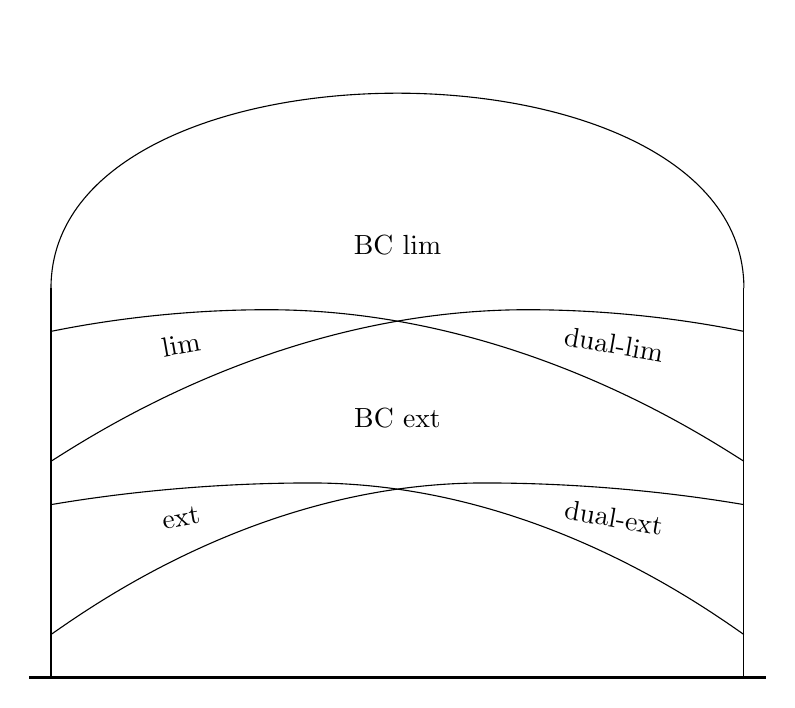
\begin{tikzpicture}
\pgftransformscale{.55}

%% Horizontal bar
\draw[very thick] (8.5,0) -- (-8.5,0);

% BC lim
\draw (-8,0) -- (-8,9);
\draw (-8,9) .. controls (-8,15) and (8,15) .. (8,9);
\draw (8,0) -- (8,9);
\node at (0,10) {BC lim};

% lim
\draw (-8,8) parabola bend (-3,8.5) (8,5);
\node[rotate=10] at (-5,7.7) {lim};

% dual-lim
\draw (-8,5) parabola bend (3,8.5) (8,8);
\node[rotate=-10] at (5,7.7) {dual-lim};

% BC ext
\node at (0,6) {BC ext};

% ext
\draw (-8,4) parabola bend (-2,4.5) (8,1);
\node[rotate=10] at (-5,3.7) {ext};

% dual-ext
\draw (-8,1) parabola bend (2,4.5) (8,4);
\node[rotate=-10] at (5,3.7) {dual-ext};

\end{tikzpicture}
\end{center}
\end{mdframed}
\end{samepage}

\begin{proof}
(1)-strictness follows with the existence of $L_a$. \\
(2)-strictness follows with \emph{closure under negation and alphabet permutation}, $L_a$ and \cref{gen:extInBCext}. \\
(3) follows with \emph{closure under suffix-independence, negation, union and change of final states} and \cref{gen:staiger-wagner}. \\
(4)-strictness follows with the existance of $L'_a$. \\
(5)-strictness follows with \emph{closure under negation and alphabet permutation}, $L'_a$ and \cref{gen:extInBCext}.
\end{proof}

Closure under suffix-independence is a very strong property, as can be seen in \cref{gen:R-suffix-indep->single-state-loops}. Note that we only needed this property in \cref{gen:main-theorem-inclusions} for the $\BC \ext \Lang = \lim \cap \dlim \Lang$ equality. However, without this equality, we don't have an easy connection between $\ext \Lang$ and $\lim \Lang$. We can have $\ext \Lang(\mathtext{finite}) \supseteq \lim \Lang(\mathtext{finite})$ as can be seen in \cref{lang:finite}. Or there are even cases where there is no inclusion in any direction, e.g. see \cref{gen:example:ext<->lim}.

Without the separating languages $L_a$, $L'_a$ from \cref{gen:main-theorem-inclusions}, we formulate a bit less restrictive version:
\begin{lemma}
Let $\Lang$ be closed under suffix-independence, negation, union, change of final states. Then
\[ \ext \cap \dext \Lang \subseteq
\ext \cup \dext \Lang \subseteq
\BC \ext \Lang =
\lim \cap \dlim \Lang \subseteq
\lim \cup \dlim \Lang \subseteq
\BC \lim \Lang . \]
\begin{proof}
The only non-obvious relation is $\BC \ext \Lang = \lim \cap \dlim \Lang$. This follows with \cref{gen:staiger-wagner}.
\end{proof}
\end{lemma}

%S406.1: TODO...
%S402: TODO...

\

In this section, we have seen some generic cases where we get the expected inclusion diagram as in \cref{gen:main-theorem-inclusions} or parts of it. However, we have also seen several examples where we have different relations. We introduced some closure properties on $\Lang$ which lead to the expected results. Most importantly is probably the closure of final states in many cases. The closure under negation, union or intersection is given for most $*$-language classes.


\subsection{Kleene closure}
\label{gen:section:kleene}

The $\Kleene$ language class operator is a bit disconnected from the study so far on $\ext$ and $\lim$. For the class of regular $*$-languages, we have the equality
\[ \Kleene \Langreg = \BC \lim \Langreg \]
as it was shown in \cref{reg-omega-lang}.

We will now study this relation for arbitrary language classes $\Lang$.

We will see that we need a somewhat stronger closure property than what we had earlier.

%\subsection{Kleene-star $= \BC \lim$}
\begin{lemma}
\label{gen:kleene-star}
Let $\Lang$ be closed under change of final states for all deterministic simplified automata. Then
\[ \Kleene \Lang \subseteq \BC \lim \Lang . \]

\begin{proof}
%S407: TODO...
%S306, S306.1:
Let $U,V \subseteq \Sigma^*$, $U\cdot V^* \in \Lang$. Look at the non-deterministic automaton $\A$ defined as:
\[
  \begin{tikzpicture}[%
    >=stealth,
	shorten >=1pt,
	node distance=2cm,
    auto,
  ]
    \node (U)              {$U$};
    \node (V) [right of=U] {$V \odot$};

    \path[->] (U) +(-1,0) edge (U)
              (U)         edge              node {$\epsilon$} (V)
              (V)         edge  [loop above]       node {} ()
              ;
  \end{tikzpicture}
\]

Then we have $L^\omega_{\text{Büchi}}(\A) = U \cdot V^\omega$.

Let us construct deterministic automata for $\A$ so that we can formulate 'V will be visited and not be left anymore' and 'finite states of the V-related automaton will be visited infinitely often' (or '$UV^*$ will be visited infinitely often').

In a constructed automaton, we must be able to tell wether we are in $U$ or we deterministically have been in $U$ the previous state. In a state power set construction, we can tell wether we are deterministically in $U$ or not. If we are non-deterministic and we may be in both $U$ or $V$ and we get an input symbol which determines that we have been in $U$, we might not be able to tell from the following power set.

\textbf{Example}:

Let $U = (a+b)^*$, $V = \Set{b}$. I.e. $UV^\omega = \Set{\alpha \in \Set{a,b}^\omega}{\text{at one point in $\alpha$, there are only $b$s}}$. The non-deterministic automaton is:
\[
  \begin{tikzpicture}[%
    >=stealth,
	shorten >=1pt,
	node distance=2cm,
    auto,
  ]
    \node[state] (1)              {$1$};
    \node[state,double] (2) [right of=1] {$2$};
	
    \path[->]
    (1) +(-1,0) edge (1)
    (1) edge [loop above] node {$a,b$} ()
    (1) edge node {$\epsilon$} (2)
    (2) edge [loop above] node {$b$} ()
    ;
  \end{tikzpicture}
\]

Powerset construction: The initial state is $\Set{1,2}$. Then we have:
\begin{itemize}
\item $\Set{1,2} \overset{a}\rightarrow \Set{1,2}$
\item $\Set{1,2} \overset{b}\rightarrow \Set{1,2}$
\end{itemize}
This gives the $*$-language $\Set{a,b}^*$ and we cannot formulate $UV^\omega$ in any way from there.

In the construction, when we got the $a$ from $\Set{1,2}$, we knew that we have been deterministically in $1$, i.e. in $U$. We loose this information. To keep it, we introduce another state flag which exactly says wether we have determined that we have been in $U$. Thus, we construct an automaton with the states $\Power(Q) \times \B_{\text{det. been in $U$}}$, where $Q$ are the states from $\A$.

For the example, we get the initial state $(\Set{1,2},1)$. Then we have:
\begin{itemize}
\item $(\Set{1,2},1) \overset{a}\rightarrow (\Set{1,2},1)$
\item $(\Set{1,2},1) \overset{b}\rightarrow (\Set{1,2},0)$
\item $(\Set{1,2},0) \overset{a}\rightarrow (\Set{1,2},1)$
\item $(\Set{1,2},0) \overset{b}\rightarrow (\Set{1,2},0)$
\end{itemize}
This is the automaton
\[
  \begin{tikzpicture}[%
    >=stealth,
	shorten >=1pt,
	node distance=2cm,
    auto,
  ]
    \node[state] (1)              {$\Set{1,2},1$};
    \node[state] (2) [right of=1] {$\Set{1,2},0$};

    \path[->]
    (1) +(-1.5,0) edge (1)
    (1) edge [loop above] node {$a$} ()
    (1) edge [bend left] node {$b$} (2)
    (2) edge [bend left] node {$a$} (1)
    (2) edge [loop above] node {$b$} ()
    ;
  \end{tikzpicture}
\]

When we mark all states from $V$ and where we have not been deterministically in $U$ as final, this as a co-Büchi automaton gives exactly the condition 'V will be visited and not be left anymore'. Let $L_E$ be the $*$-language of this automata. Note that $L_E \neq UV^*$ in general and esp. in the example.

When we mark the final states as in the original non-deterministic automata, no matter about $\B_{\text{det. been in $U$}}$, with Büchi-acceptance, we get the condition '$UV^*$ will be visited infinitely often'. This is just $\lim UV^*$.

Together, we get $UV^\omega$, i.e.:
\[ \lim UV^* \cap \dlim L_E = UV^\omega \]

Given the \emph{closure under change of final states for all deterministic simplified automata}, we have $L_E \in \Lang$. Then, it follows
\[ \Set{ \bigcup_{i=1}^n U_i \cdot V_i^\omega}{U_i,V_i \subseteq \Sigma^*, U_i\cdot V_i^* \in \Lang} = \Kleene \Lang \subseteq \BC \lim \Lang . \]
\end{proof}
\end{lemma}

Note that the idea in this proof can probably be generalized into a general non-deterministic Büchi to deterministic Muller automaton conversion.

%S306.3:
\begin{lemma}
Let $\Lang$ be closed under change of final states. Then
\[ \lim \Lang \subseteq \Kleene \Lang . \]
\begin{proof}
Let $\A$ be a minimal deterministic automaton with final states $F$ such that $L^*(\A) \in \Lang$. Define $\tilde L := L^\omega_{\text{Büchi}}(\A)$.

For all finite states $q \in F$: If $q$ is not part of a strongly connected component (SCC), we can ignore it. Let $S$ be the SCC where $q \in S$. Then the set of all $\alpha \in \Sigma^\omega$ which are infinitely often in $q$ can be described as $U_q \cdot V_q^\omega$, where $U_q$ is the set of words so that we arrive in $q$ and $V_q$ is the set of words so that we get from $q$ to $q$. Both sets are obviously regular and because of the \emph{closure of change of final states} (by letting $q$ be the only final state), we have $U_q V_q^* \in \Lang$.

Thus,
\[ \tilde L = L^\omega_{\text{Büchi}}(\A) = \bigcup_{q \in F} U_q V_q^\omega . \]
%
%Obviously, $\Kleene \Lang$ is closed under union.
%
%Show that Kleene-Closure is closed under negation. (S306.5) (Follows with non-det Büchi complementation but a more generic proof might be useful.)
%Let's show that Kleene-Closure is closed under negation: Let $\tilde L \in \Kleene \Lang$. With \cref{gen:kleene-star}, we have that $\tilde L \in \BC \lim \Lang$.
\end{proof}
\end{lemma}

Open at this point is the stronger inclusion $\BC \lim \Lang \subseteq \Kleene \Lang$.

We see that the relation between $\BC \lim \Lang$ and $\Kleene \Lang$ is not so obvious for arbitrary $*$-language classes.


\subsection{Congruence based language classes}
\label{gen:R}

\subsubsection{Introduction}
\label{gen:R-automata}

\begin{mydef}
We define $\Lang(R)$ for an equivalence relation $R\subseteq\Sigma^* \times \Sigma^*$
\[ \Lang^*(R) := \Set{L \subseteq \Sigma^*}{L \text{ is finite union of $R$-equivalence-classes}} . \]
\end{mydef}

Examples of such language classes are $n$-locally testable ($\LT_n$, \cref{lang:LT}), $k,r$-locally threshold testable ($\LTT_r^k$, \cref{lang:LTT}) or $n$-piecewise testable ($\PT_n$, \cref{lang:PT}) languages. The exact definition is given in their related section. At their definition, the word-relation basically tells wether a local test / piece-wise test can see a difference between two words.

%S307
If a language class $\Lang(R)$ is defined as finite union of equivalence classes of a relation $R \subseteq \Sigma^* \times \Sigma^*$ and
\begin{itemize}
\item the set of equivalent classes of $R$ is finite,
\item $R$ is a congruence relation, i.e. also $(v,w) \in R \ \Leftrightarrow \ (va,wa) \in R \ \ \forall a \in \Sigma$
\end{itemize}
then we can construct a canonical deterministic automaton $\A_R$ which has $S_R := \Sigma^* / R$ as states, $\left<\epsilon\right>_R$ is the initial state and the transitions are according to concatenation. Call this an $R$-automaton.

The $\LT_n$, $\LTT^k_r$ and $\PT_n$ language classes have the above properties and thus such related canonical automaton.

The set of all such $R$-automata, varying in the final state set, is isomorphic to $\Lang(R)$. We have
\[ \Lang^*(R) = \Set{L^*(\A_R(F))}{F \subseteq S_R} =: \Lang^*(\A_R) . \]

Obviously, by construction, such language classes are all \emph{closed under change of final states}. Obviously, $\Lang^*(R)$ is also closed under \emph{negation, union and intersection} (via negating, merging or intersecting the final state set of related automata). \emph{Closure under suffix-independence} doesn't directly follow from this --- we see some counter example later.

\begin{mydef}
Analogously for $\omega$, we get the set of $R$-E-automata with the $\omega$-language-class
\[ \Lang^\omega_E(\A_R) := \Set{L^\omega_E(\A_R(F))}{F \subseteq S_R} , \]
$R$-Büchi-automata and
\[ \Lang^\omega_{\text{Büchi}} (\A_R) := \Set{L^\omega_\text{Büchi}(\A_R(F))}{F \subseteq S_R} , \]
$R$-Muller-automata and
\[ \Lang^\omega_{\text{Muller}} (\A_R) := \Set{L^\omega_\text{Muller}(\A_R(\F))}{\F \subseteq 2^{S_R}} . \]
\end{mydef}


\subsubsection{Classification}

With this preparation, we get some obvious results:
\begin{lemma}
\label{gen:R:closurelemma}
$\Lang(R)$ is closed under negation, union, intersection and change of final states.
\begin{proof}
The closure under negation, union, intersection follows directly from negation, union and intersection of the final state set in $R$-automata.

For any language $L \in \Lang(R)$, the minimal deterministic automaton $\A_L$ is a subset of an $R$-automaton. Thus, any change of final states can be transferred to the $R$-automaton and we stay in the language class. I.e. $\Lang(R)$ is closed under change of final states.
\end{proof}
\end{lemma}

\begin{example}
There is an $R$ such that $\Lang(R)$ is \textbf{not} closed under suffix-independence.
\begin{proof}
Look at the transition graph over $\Sigma := \Set{a,b}$:
\[
  \begin{tikzpicture}[%
    >=stealth,
	shorten >=1pt,
	node distance=2cm,
    auto,
  ]
    \node[state] (0)              {$0$};
    \node[state] (1) [right of=0] {$1$};
    \node[state] (2) [below of=0] {$2$};

    \path[->]
    (0) +(-1.5,0) edge (0)
    (0) edge [bend left] node {$a$} (1)
    (0) edge [bend right] node {$b$} (2)
    (1) edge [bend left] node {$a$} (2)
    (1) edge [bend left] node {$b$} (0)
    (2) edge [loop below] node {$a,b$} ()
    ;
  \end{tikzpicture}
\]
Define the congruence relation $R \subseteq \Sigma^* \times \Sigma^*$ as $(v,w) \in R \ :\Leftrightarrow \ v,w$ end up in the same state. Then, the above transition graph is exactly the $R$-automaton.

If $1$ is the only final state, this is the language $L_1 = a(ba)^*$. With suffix independence, we get the language $L_1 \cdot \Sigma^* = a \Sigma^*$.

$a \Sigma^* \not\in \Lang(R)$, thus $\Lang(R)$ is not \emph{closed under suffix-independence}.

Furthermore, $\ext L_1 = a \Sigma^\omega$. Marking $0$ or $1$ as final state in a $R$-Büchi-automaton accepts the language $\tilde L_1 := \Set{(ab)^\omega}$. Marking $2$ as final state accepts the language $\tilde L_2 := (ab)^* (b | aa) \Sigma^\omega$. Then, $\lim \Lang(R) = \Set{\emptyset, \tilde L_1, \tilde L_2, \tilde L_1 \cup \tilde L_2}$. And we have $\ext L_1 \not\in \lim \Lang(R)$. But we also have $\tilde L_1 \not\in \ext \Lang(R)$.
\end{proof}
\end{example}

In the rest of this section, we show some equalities:
\begin{itemize}
\item $\Lang^\omega_E(\A_R) = \ext \Lang(R)$ (\cref{gen:lang_omega_e})
\item $\Lang^\omega_{\text{Büchi}}(\A_R) = \lim \Lang(R)$ (\cref{gen:lang_omega_buechi})
\item $\Lang^\omega_{\text{Muller}}(\A_R) = \BC \lim \Lang(R)$ (\cref{gen:lang_omega_muller})
\item $\BC \lim \Lang(R) \cap \ext \Langreg = \ext \Lang(R)$ (\cref{gen:R-bclim-cap-ext})
\end{itemize}

We will see that all those equations hold for all $R$, i.e. also for $\Lang(\LT_n)$, $\Lang(\LTT^k_r)$ and $\Lang(\PT_n)$.

Note that we still don't necessarily have $\ext \Lang(R) \subseteq \lim \Lang(R)$. The \cref{gen:example:ext<->lim} also applies here.

We will also see that
\[ \BC \lim \Lang(R) \cap \lim \Langreg = \lim \Lang(R) \]
is not always the case. We will give an alternative characterization of this property (\cref{gen:postfix-loop-det=limAndBclim}).

Again, a bit more special is the relation
\[ \lim \Lang(R) \cap \dlim \Lang(R) = \BC \ext \Lang(R) \]
(\cref{gen:R-staiger-wagner}).

\begin{lemma}
%\subsection{$\Lang^\omega_E(\A_R) = \ext \Lang(R)$}
%S307.2,S307.3
\label{gen:lang_omega_e}
\[ \Lang^\omega_E(\A_R) = \ext \Lang(R) \]
\begin{proof}
Let $L = \bigcup_i \left< w_i\right>_R, L \in \Lang(R)$. Then
\begin{align*}
& L^\omega = \ext L \\
\Leftrightarrow \ & L^\omega = \Set{\alpha \in \Sigma^\omega}{\exists n \colon \alpha[0,n] \in \bigcup_i \left< w_i\right>_R} \\
\Leftrightarrow \ & L^\omega = \Set{\alpha \in \Sigma^\omega}{\exists n \colon \delta_{\A_R}(\alpha[0,n]) \in \Set{\left< w_i\right>_R \subseteq S_R}{i}} \\
\Leftrightarrow \ & L^\omega = L^\omega(\A^E_R(\Set{\left< w_i\right>_R \subseteq S_R}{i}))
\end{align*}
\end{proof}
\end{lemma}

\begin{lemma}
%\subsection{$\Lang^\omega_{\text{Büchi}}(\A_R) = \lim \Lang(R)$}
%S307.2,S307.3
\label{gen:lang_omega_buechi}
\[ \Lang^\omega_{\text{Büchi}}(\A_R) = \lim \Lang(R) \]
\begin{proof}
Let $L = \bigcup_i \left< w_i\right>_R, L \in \Lang(R)$. Then
\begin{align*}
& L^\omega = \lim L \\
\Leftrightarrow \ & L^\omega = \Set{\alpha \in \Sigma^\omega}{\exists^\infty n \colon \alpha[0,n] \in \bigcup_i \left< w_i\right>_R} \\
\Leftrightarrow \ & L^\omega = \Set{\alpha \in \Sigma^\omega}{\exists^\infty n \colon \delta_{\A_R}(\alpha[0,n]) \in \Set{\left< w_i\right>_R \subseteq S_R}{i}} \\
\Leftrightarrow \ & L^\omega = L^\omega(\A^{\text{Büchi}}_R(\Set{\left< w_i\right>_R \subseteq S_R}{i}))
\end{align*}
\end{proof}
\end{lemma}

\begin{lemma}
%\subsection{$\Lang^\omega_{\text{Muller}}(\A_R) = \BC \lim \Lang(R)$}
%S307.2,S307.3
\label{gen:lang_omega_muller}
\[ \Lang^\omega_{\text{Muller}}(\A_R) = \BC \lim \Lang(R) \]
\begin{proof}
Any $L^\omega \in \BC \lim \Lang(R)$ can be described by $\BC 2^{S_R}$. $2^{2^{S_R}}$ is also finite. Thus, any $A \in \BC 2^{S_R}$ can be represented in $2^{2^{S_R}}$. This is exactly an acceptance condition in Muller.
\end{proof}
\end{lemma}


When we compare the outer $\ext \Langreg$ (inside $\BC \lim \Langreg$, i.e. all regular $\omega$-languages) which is clearly a superset of $\ext \Lang$ and the inner whole class $\BC \lim \Lang$, a natural question is wether $\BC \lim \Lang \cap \ext \Langreg = \ext \Lang$. This is the case for $\Lang(R)$ as shown below.

\begin{lemma}
%\subsection{$\BC \lim \Lang(R) \cap \ext \Langreg = \ext \Lang(R)$}
%S307.6,S307.7,S307.8
\label{gen:R-bclim-cap-ext}
\[ \BC \lim \Lang(R) \cap \ext \Langreg = \ext \Lang(R) \]

\begin{proof}
We have $\ext \Lang(R) \subseteq \ext \Langreg$ and $\ext \Lang(R) \subseteq \BC \lim \Lang(R)$. Thus, "$\supseteq$" is shown.

Now, we show "$\subseteq$". Let $L^\omega \in \BC \lim \Lang(R) \cap \ext \Langreg$. Because $L^\omega \in \ext \Langreg$, there is an E-automaton $\A^E$ which accepts $L^\omega$. We can assume that $\A^E$ is deterministic (with \cref{gen:e-determinism}).

We must find an $R$-E-automaton which accepts $L^\omega$. We will call it the $\overline{\A}^M$ E-automaton and will construct it in the following.

Let $\A^M$ be the deterministic $R$-Muller-automaton for $L^\omega$ (according to \cref{gen:R-automata} and \cref{gen:lang_omega_muller}). Without restriction, there are no final state sets in $\A^M$ which are not loops. Then, $\overline{\A}^M$ has the same states and transitions as $\A^M$.

Look at a final state $q^E$ of $\A^E$. Without restriction, we can assume that there is no path that we can reach multiple final states at once. Let $L_{q^E}$ be all words which reach $q^E$ exactly once at the end.

Let $w \in L_{q^E}$.
%In $\A^M$, after $w$, we reached a state where anything that follows will eventually reach a SCC where any possible looping subset is an element of the final state set of $\A^M$ and there is no way out of the SCC.
%Look at some SCC $S$ in $\A^M$. Let $q \in S$. Let $\F$ be the subset of the finite state set of $\A^M$ so that $q \in F$ for all $F \in \F$, i.e. $F \cap S \neq \emptyset$. We can ignore all $F$ which are not a loop because they would not accept anything because they cannot be reached infinitely often. Because $S$ is a SCC and $F$ is a loop, we also get $F \subseteq S$.
Let $q$ be the state in $\A^M$ which is reached after $w$. Let $S$ be the set of states in $\A^M$ which can be reached from $q$.
%Let $\F$ be the subset of the finite state set of $\A^M$ so that $F \cap S \neq \emptyset$ for all $F \in \F$. We also get $F \subseteq S$.

Then, $\A^M$ accepts all words in $L_q \cdot L_{q,S}^\omega$, where $L_q$ is the set of words to $q$ and $L^\omega_{q,S}$ is the set of words of possible infinite postfixes after $q$ in $S$ so that they are accepted.
%loops $q\rightarrow q$ in $\F$.
Any word with a prefix in $L_q$, which is not in $L_q \cdot L^\omega_{q,S}$, will not be accepted by $\A^M$ because $\A^M$ is deterministic. Also, because $L_{q^E} \cap L_q \neq \emptyset$ and $L_{q^E} \cdot \Sigma^\omega \subseteq L^\omega$ and $L_q \cdot L^\omega_{q,S} \subseteq L^\omega$, we get $L^\omega_{q,S} \neq \emptyset$.

Assuming $L^\omega_{q,S} \neq \Sigma^\omega$. Then we would have $L^\omega \not\in \ext \Langreg$, which is a contradiction. I.e. $L^\omega_{q,S} = \Sigma^\omega$.

Thus, $\A^M$ accepts all words in $L_q \cdot \Sigma^\omega$. Mark $q$ as a final state in $\overline{\A}^M$. Thus, $\overline{\A}^M$ E-accepts all words in $L_q \cdot \Sigma^\omega \subseteq L^\omega$.

%For any state $\tilde q$ in $\A^M$ which is not marked as a final state in the previously described way, all states in $\A^E$ after words in $L_{\tilde q}$ are not final states in $\A^E$. Thus, all words not in $L^\omega$ are not accepted by $\overline{\A}^M$.

Because we did this for all final states in $\A^E$, there is no $\alpha \in L^\omega$ which is not accepted by $\overline{\A}^M$. I.e., the $R$-E-automata $\overline{\A}^M$ accepts exactly $L^\omega$. I.e. $L^\omega \in \ext \Lang(R)$.
\end{proof}
\end{lemma}

In fact, we actually have shown $\BC \lim \Lang \cap \ext \Langreg = \ext \Lang$ for any $\Lang \subseteq \Langreg$.


We are also interested in the equality $\BC \lim \Lang \cap \lim \Langreg = \lim \Lang$ for some $*$-language class $\Lang \subseteq \Langreg$. This is a connection between the outer $\lim \Langreg$ (inside $\BC \lim \Langreg$) which is clearly a superset of $\lim \Lang$ and the inner whole class $\BC \lim \Lang$. It turns out that this is not always the case and not as straightforward as in the $\ext$ case in \cref{gen:R-bclim-cap-ext}.

We have $\lim \Lang \subseteq \lim \Langreg$ and $\lim \Lang \subseteq \BC \lim \Lang$. Thus, "$\supseteq$" does hold in all cases.

\begin{example}
\label{gen:bcLimLReg-and-limL:counter-example}
The equality does not hold for any $\Lang$.
\begin{proof}
Let $\Sigma = \Set{a,b}$,
\[ L_a := (b^* a^+) (b^+ a^+)^* , \ \ \ L_b := b^* (a^+ b^+)^* \ \ \ \text{and} \ \ \ \Lang := \Set{L_a,L_b} . \]
Then, $\lim L_a$ is the set of words where $a$ occurs infinitely often and $\lim L_b$ is the set of words where $b$ occurs infinitely often. Then, $L_\omega := \lim L_a \cap \lim L_b \in \BC \lim \Lang$. Also, let
\[ L_{ab} := (a^* b^+ a)^* . \]
Then, $\lim L_{ab}$ is the set of words where both $a$ and $b$ occurs infinitely often. Thus, $\lim L_{ab} = L_\omega$. Obviously, we also have $L_{ab} \in \Langreg$. Thus, $L_\omega \in \BC \lim \Lang \cap \lim \Langreg$. But we can also see that $L_\omega \not\in \lim \Lang$.
\end{proof}
\end{example}

Thus, we need some conditions on $\Lang$ for the equality. Here, we will study the class $\Lang(R)$. We will introduce a property on $\Lang(R)$ where we can show the equality. The idea of this property is coming from the study of this equality in terms of automata. Let $L_\omega \in \BC \lim \Lang(R)$. Then there is a representing $R$-Muller-automaton $\A_M$ for $L_\omega$. Let also $L_\omega \in \lim \Langreg$. Then there is representing deterministic Büchi automaton $\A_r$ for $L_\omega$. We want to show that $L_\omega \in \lim \Lang(R)$. I.e. we are searching for a representing deterministic automaton whose language is in $\Lang(R)$ and where the Büchi-acceptance gives us $L_\omega$. Because the $R$-Büchi-automaton is the canonical deterministic Büchi automaton for $\Lang(R)$, we must be able to construct such $R$-Büchi-automaton $\A_B$ for $L_\omega$. Let us look at the product automaton $\A_M \times \A_r$ and determine from there the final state set of $\A_B$. $\A_M$ already has the right transition graph. $\A_r$ has the Büchi acceptance. So, when looking at the product automaton, we try to find the loops in $\A_M$ which match a final state in $\A_r$. $\A_r$ might be bigger than $\A_M$ and it doesn't seem clear wether the Muller final state sets of $\A_M$ can be translated to a Büchi final state set. However, when we say that each SCC in $\A_M$ has exactly one loop, there is no inconclusiveness about wether there is a Büchi final state in this SCC in $\A_B$ or not. We will formulate this formally below. So, if we have that property on $\A_M$, i.e. on $\Lang(R)$, we can construct $\A_B$ and thus we have the equality.

\begin{mydef}
\label{gen:def:infinity-postfix-independent}
For $\alpha \in \Sigma^\omega$, let $\overrightarrow \alpha \in (\Sigma^* / R)^\omega$ be the state sequence we run through with $\alpha$ and thus $\Inf(\overrightarrow \alpha) \subseteq \Sigma^*/R$ those states which are visited infinitely often.

If for every $L \in \Lang(R)$, there is an inclusion function $B_L \colon \Sigma^*/R \rightarrow \B$ such that for every $\alpha \in \Sigma^\omega$, we have
\[ \alpha \in L \ \ \ \Leftrightarrow \ \ \ \exists q \in \Inf(\overrightarrow \alpha) \colon B_L(q) = 1 . \]
Also, for every $s \not\in \Inf(\overrightarrow \alpha)$,
\[ B_L(s) = B_L(q) \ \ \ \forall q \not\in \Inf(\overrightarrow \alpha) \]
and
\[ B_L(s) \neq B_L(q) \ \ \ \forall q \in \Inf(\overrightarrow \alpha) . \]

If such $B_L$ always exists, we call $\Lang$ \defword{infinity-postfix-independent}.
\end{mydef}

This definition is as general as possible. It is also well defined if there are an infinity number of equivalence classes of $R$. Thus, $\Lang(R)$ doesn't need to be regular. Also, in that case, there might be an $\alpha \in \Sigma^\omega$ with $\Inf(\overrightarrow \alpha) = \emptyset$.

If $\Lang(R)$ is regular and we look at an $R$-$\omega$-automaton, it basically says that when we visit some state infinitely often, it determines in what loop we are and we cannot switch the loop. Formally:

\begin{lemma}
\label{gen:infPostfixIndep-AutLoops}
Let $R$ be a congruence relation with a finite number of equivalence classes. $\Lang(R)$ is \emph{infinity-postfix-independent} exactly if and only if every SCC $Q$ in the $R$-automata (as defined in section \ref{gen:R-automata}) has exactly one looping subset, i.e. $Q$ itself is the only loop in $Q$.
\begin{proof}
$S_R := \Sigma^*/R$ are the states of the $R$-automata. Let $Q \subseteq S_R$ be any SCC. Let $\tilde L \in \BC \lim \Lang(R)$. Let $\A_M$ be the $R$-Muller-automaton accepting $\tilde L$.

'$\Rightarrow$': Let $\Lang(R)$ be \emph{infinity-postfix-independent}. Then, for $L$, we have an inclusion function $B_L \colon S_R \rightarrow \B$. If there is an accepting loop $Q' \subseteq Q$ in $\A_M$, it means that every $\alpha \in \tilde L$ which ends up in $Q'$ is accepted, thus there is a $q' \in Q'$ with $B_L(q') = 1$. Because we can loop through all of $Q$ and thus construct $\beta \in \Sigma^\omega$ with $\Inf(\overrightarrow \beta) = Q$, we get $B_L(q) = 1$ for all $q \in Q$. Thus, all possible loops in $Q$ will accept. This was general for any SCC and any language $\tilde L \in \BC \lim \Lang(R)$. Because this is a Muller-automaton, this can only be if $Q$ itself is the only loop. Otherwise we can have both an accepting loop and a non-accepting loop in $Q$ which is a contradiction.

'$\Leftarrow$': The SCC $Q$ has exactly one looping subset. This is $Q$ itself. Assuming $Q$ is accepting in $\A_M$. Then define $B_L(q) = 1$ for all $q \in Q$, otherwise $B_L(q) = 0$. This $B_L \colon S_R \rightarrow \B$ has the needed properties, thus $\Lang(R)$ is \emph{infinity-postfix-independent}.
\end{proof}
\end{lemma}

For piecewise testable languages, this is the case. See \cref{lang:PT}.

For locally testable languages, this is \emph{not} the case. Depending on the ending of $\alpha[0,n]$, we can switch through different equivalence classes and visit different loops. See \cref{lang:LT}.

\begin{example}
There is an $R$ so that $\Lang(R)$ is not \emph{infinity-postfix-independent} and
\[ \BC \lim \Lang(R) \cap \lim \Langreg \neq \lim \Lang(R) . \]
\begin{proof}
If we take the \cref{gen:bcLimLReg-and-limL:counter-example}: For $v,w \in \Set{a,b}^*$, let $v =_R w \ :\Leftrightarrow \ v,w$ end up with the same symbol. I.e., the equivalence classes are $\left<\epsilon\right>, \left<a\right>, \left<b\right>$.

The $R$-automata is
\[
  \begin{tikzpicture}[%
    >=stealth,
	shorten >=1pt,
	node distance=2cm,
    auto,
  ]
    \node[state] (0)              {$\left<\epsilon\right>$};
    \node[state] (2) [right of=0] {$\left<b\right>$};
    \node[state] (1) [above of=2] {$\left<a\right>$};

    \path[->]
    (0) +(-1.5,0) edge (0)
    (0) edge [bend left] node {$a$} (1)
    (0) edge [bend right] node {$b$} (2)
    (1) edge [loop right] node {$a$} ()
    (1) edge [bend left] node {$b$} (2)
    (2) edge [bend left] node {$a$} (1)
    (2) edge [loop right] node {$b$} ()
    ;
  \end{tikzpicture}
\]

From \cref{gen:bcLimLReg-and-limL:counter-example}, we have $L_a = \left<a\right>$ and $L_b = \left<\epsilon\right> \cup \left<b\right>$ and $\Lang = \Set{L \in \Lang(R)}{\#L = \infty}$ (only the infinity $L \in \Lang(R)$ matter for $\lim$). We also see from the $R$-automata that there is no way to mark states as final states for Büchi-acceptance so that we get the condition "both $a$ and $b$ occur infinitely often". Via Muller, we just mark the loop $\Set{\left<a\right>,\left<b\right>}$ as final. I.e. $\lim L_{ab} \not\in \lim \Lang(R)$ but $\lim L_{ab} \in \BC \lim \Lang(R)$ and as shown in \cref{gen:bcLimLReg-and-limL:counter-example}, $\lim L_{ab} \in \lim \Langreg$. Thus, $\BC \lim \Lang(R) \cap \lim \Langreg \neq \lim \Lang(R)$.
\end{proof}
\end{example}

This example can actually be extended to be the $\Lang(LT_2)$ class and generalized to any $\Lang(LT_n)$. I.e. for all $n \in \N$, $\Lang(LT_n)$ is not \emph{infinity-postfix-independent} and
\[ \BC \lim \Lang(LT_n) \cap \lim \Langreg \neq \lim \Lang(LT_n) . \]

When studying the \emph{infinity-postfix-independence} property in more detail, we get the surprising result:

\begin{lemma}
\label{gen:BClimR=limR}
Let $R$ be a congruence relation with a finite number of equivalence classes. Let $\Lang(R)$ be \emph{infinity-postfix-independent}. Then %exactly if and only if
\[ \BC \lim \Lang(R) = \lim \Lang(R) . \]
\begin{proof}
$S_R := \Sigma^*/R$ are the states of the $R$-automata. Let $Q \subseteq S_R$ be any SCC. Let $\tilde L \in \BC \lim \Lang(R)$. Let $\A_M$ be the $R$-Muller-automaton accepting $\tilde L$.

%'$\Rightarrow$':
%Let $\Lang(R)$ be \emph{infinity-postfix-independent}. Then,
For $L$, we have an inclusion function $B_L \colon S_R \rightarrow \B$. If there is an accepting loop $Q' \subseteq Q$ in $\A_M$, it means that every $\alpha \in \tilde L$ which ends up in $Q'$ is accepted, thus there is a $q' \in Q'$ with $B_L(q') = 1$. Because we can loop through all of $Q$ and thus construct $\beta \in \Sigma^\omega$ with $\Inf(\overrightarrow \beta) = Q$, we get $B_L(q) = 1$ for all $q \in Q$. Thus, all possible loops in $Q$ will accept. In an $R$-Büchi-automata $\A_B$, we can mark all states of $Q$ as final states. This was for any SCC $Q$, thus $\A_B$ will accept exactly iff $\A_M$ accepts. Thus we have $\tilde L \in \lim \Lang(R)$. This was for any $\tilde L$, i.e. $\BC \lim \Lang(R) = \lim \Lang(R)$.
%
%'$\Leftarrow$': Let $\BC \lim \Lang(R) = \lim \Lang(R)$. Assuming $Q$ has a final state $q \in Q$ in the $R$-Büchi-automata for $\tilde L$. Let $\alpha \in \Sigma^\omega$ so that $q \in \Inf(\overrightarrow \alpha)$.
%
%TODO ...
\end{proof}
\end{lemma}

%\subsection{$\BC \lim \Lang(R) \cap \lim \Langreg = \lim \Lang(R)$}
%S307.6,S307.8
\begin{lemma}
\label{gen:bcLimLReg-and-limL}
Let $R$ be a congruence relation with a finite number of equivalence classes. Let $\Lang(R)$ be \emph{infinity-postfix-independent}. Then
\[ \BC \lim \Lang(R) \cap \lim \Langreg = \lim \Lang(R) . \]

\begin{proof}
In \cref{gen:BClimR=limR}, we showed that we have $\BC \lim \Lang(R) = \lim \Lang(R)$. Because $\lim \Lang(R) \subseteq \lim \Langreg$, we directly get the claimed equality.
\end{proof}
\end{lemma}

%This proof is loosely analogue to the proof in \ref{gen:R-bclim-cap-ext}.

%It was already shown that "$\supseteq$" always holds.

%Now, we show "$\subseteq$". Let $L^\omega \in \BC \lim \Lang(R) \cap \lim \Langreg$. Because $L^\omega \in \lim \Langreg$, there is an Büchi-automaton $\A^B$ which accepts $L^\omega$. We can assume that $\A^B$ is deterministic (with \ref{gen:e-determinism}).

%We must find an $R$-Büchi-automaton which accepts $L^\omega$. We will call it the $\overline{\A}^M$ Büchi-automaton and will construct it in the following.

%Let $\A^M$ be the deterministic $R$-Muller-automaton for $L^\omega$ (according to \ref{gen:R-automata} and \ref{gen:lang_omega_muller}). Without restriction, there are no final state sets in $\A^M$ which are not loops. Then, $\overline{\A}^M$ has the same states and transitions as $\A^M$.

%Look at the SCC $S$ in $\A^M$. Let $q \in S$. Let $\mathcal F_q \subseteq 2^S$ be the set of final states in $\A^M$ with $q \in F$ for all $F \in \F_q$. Let $\mathcal S_q \subseteq 2^S$ be the set of loops in $S$ which include $q$.

%Case 1: $\F_q \neq \mathcal S_q$.

%Case 2: $\F_q = \mathcal S_q$.
%In that case, mark $q$ as a final state in $\overline{\A}^M$.

%For the constructed Büchi-automaton $\overline{\A}^M$, we show that it accepts exactly $L^\omega$.

%Let $\alpha \in L^\omega(\overline{\A}^M)$. Let $q$ be some final state in $\overline{\A}^M$ which is infinitely often visited by $\alpha$. Then, $\F_q = \mathcal S_q$ from the construction. I.e., no matter what loops through $q$ of the related SCC are visited infinitely often by $\alpha$, it will be accepted by $\A^M$. Thus, $\alpha \in L^\omega$.

%Let $\alpha \in L^\omega$. Then, the set of states $F$ infinitely often visited by $\alpha$ in $\A^M$ is some final state set of the Muller-automaton $\A^M$. In $\A^B$, there is a final state $\tilde q$ infinitely often visited by $\alpha$. Let $\alpha =: \prod_{i=1}^{\infty} w_i$ so that $\prod_{i=1}^{n} w_i$ ends up in $\tilde q$ in $\A^B$ for all $n \in \N$ for shortest possible $w_i$ (i.e. we don't miss any $\tilde q$). Let $S$ be the SCC in $\A^M$ where we finally end up with $\alpha$. Then, $F \subseteq S$.

%There must be a $q \in F$ so that $\F_q = \mathcal S_q$. Then, by construction of $\overline{\A}^M$, $q$ is a final state in $\overline{\A}^M$ and thus, $\alpha \in L^\omega(\overline{\A}^M)$.

%Let us show that there is such $q \in F$ by contradiction. I.e. assume there is no such $q \in F$. I.e. for all $q \in F$, $\F_q \neq \mathcal S_q$. Of course we have $F \in \F_q$ for all $q \in F$.

%Let $\mathcal P_{\tilde q}$ be the set of loops in $\A^M$ so that all words which end up looping there infinitely would also visit $\tilde q$ infinitely often in $\A^B$. Of course, all $P \in \mathcal P_{\tilde q}$ will be final state sets in $\A^M$ because $\A^B$ would accept. Define $\mathcal P_{\tilde q,S} := \Set{P \in \mathcal P_{\tilde q}}{P \subseteq S}$. No matter how much other infinte loops in $S$ we add to $\alpha$ so that we still visit some loops from $\mathcal P_{\tilde q,S}$ infinitely often, $\A^M$ and $\A^B$ will keep accepting. Thus, for $P \in \mathcal P_{\tilde q,S}$, every $P' \supseteq P$, $P' \in \mathcal S_S$, we have $P' \in \mathcal P_{\tilde q,S}$.

%For any $q \in F$, we have $\F_q \neq \emptyset$. Thus, $q$ is marked as a final state in $\overline{\A}^M$ and thus, $\overline{\A}^M$ accepts $\alpha$.

%Let us show $\F_q = \mathcal S_q$ under the condition $\F_q \neq \emptyset$. Of course we have $\F_q \subseteq \mathcal S_q$. Let $\A^B$ be the deterministic Büchi automaton for $L^\omega$ (we have $L^\omega \in \lim \Langreg$).
%Let $L_q$ be the set of words which reach $q$ in $\A^M$.
%We show the assumption by contradiction: Let $S \in \mathcal S_q$ with $S \not\in \F_q$. Let $F \in \F_q$ with $F \subseteq S$ or $F \cup S \in \F_q$ (TODO: does that exists?! -> no!).

%Let $L_{q,S} \subseteq \Sigma^*$ be the set of non-looping words from $q \rightarrow q$ in $S$, and likewise $L_{q,F} \subseteq \Sigma^*$ in $F$.

%Let $w \in L_q$, $\overline w_1 \in L_{q,F}$. Then, the infinite states visited by $w \overline w_1$ are exactly $F$. Thus, we have $w \overline w_1 \in L^\omega$.
%Let $\overline w_2 \in L_{q,S}$.
%In $\A^B$, after $w \cdot \Set{\overline w_1, \overline w_2}^\omega$, we will eventually reach a final SCC $S_B$. Let $\tilde w \in w \cdot \Set{\overline w_1, \overline w_2}^*$, so that $\tilde w$ reaches $S_B$. We have $\tilde w \cdot \Set{\overline w_1,\overline w_2}^* \cdot \overline w_1^\omega \subseteq L^\omega$.

%Let $W := \tilde w \cdot \Set{\overline w_1,\overline w_2}^*$, $W_1 := \overline w_1^+$, $W_2 := (\overline w_1^* \overline w_2 \overline w_1^*)^+$.
%Search $q_B \in S_B$ with $W \rightarrow q_B$, $q_B \xrightarrow{W_1} q_B$ and $q_B \xrightarrow{W_2} q_B$. Assuming such a $q_B$ exists with $\tilde w_0 \in W$, $\tilde w_1 \in W_1$, $\tilde w_2 \in W_2$ so that $\tilde w_0 \rightarrow q_B$, $q_B \xrightarrow{\tilde w_i} q_B$ for $i \in \Set{1,2}$. Because $\tilde w_0 \cdot \tilde w_1^\omega \in L^\omega$, there is a final state $\tilde q_B$ in $\A^B$ on the path $q_B \xrightarrow{\tilde w_1} q_B$. Then, $\beta := \tilde w_0 \cdot (\tilde w_1 \cdot \tilde w_2)^\omega$ also visits $\tilde q_B$ infinitely often, thus $\A^B$ also accepts $\beta$. In $\A^M$, $\beta$ visits exactly $F \cup S$ infinitely often. Thus, $\A_M$ does not accept $\beta$. That is a contradiction. Thus, $\F_q = \mathcal S_q$.

%TODO: Now show that such $q_B$ exists with $\tilde w_0 \in W$, $\tilde w_1 \in W_1$, $\tilde w_2 \in W_2$.

%---
%
%Note that this proof does not work for any $\A^M$. E.g. the language
%\[ \Set{\alpha \in \Set{a,b}^\omega}{\text{$a$ and $b$ do occur infinitely often in $\alpha$}} \]
%is accepted exactly by the Muller automaton
%\[
%  \begin{tikzpicture}[%
%    >=stealth,
%	shorten >=1pt,
%	node distance=2cm,
%    auto,
%  ]
%    \node[state] (1)              {$1$};
%    \node[state] (2) [right of=1] {$2$};
%
%    \path[->]
%    (1) +(-1.5,0) edge (1)
%    (1) edge [loop above] node {$a$} ()
%    (1) edge [bend left] node {$b$} (2)
%    (2) edge [bend left] node {$a$} (1)
%    (2) edge [loop above] node {$b$} ()
%    ;
%  \end{tikzpicture}
%\]
%where $\F = \Set{\Set{1,2}}$. It is not possible to find a final state set to Büchi-accept this language based on this state/transition graph, thus this automaton would not work in the proof. It is not possible to accept this language with a Muller automaton with less states, so in some way the given automaton is minimal. This demonstrates that some form of minima restriction/condition on $\A^M$ would not work for the proof.

%TODO: then show that if not (P), then not equality

The question arises wether \emph{infinity-postfix-independence} on $\Lang(R)$ is equivalent to the equality $\BC \lim \Lang(R) \cap \lim \Langreg = \lim \Lang(R)$. We have shown in \cref{gen:infPostfixIndep-AutLoops} that if $\Lang(R)$ is not \emph{infinity-postfix-independent}, there must be a SCC $Q \subseteq S_R$ with more than one loop.

\begin{example}
There is a congruence relation $R$ with a finite number of equivalence classes where $\Lang(R)$ is not \emph{infinity-postfix-independent} but we still have
\[ \BC \lim \Lang(R) \cap \lim \Langreg = \lim \Lang(R) . \]
\begin{proof}
Look at the fully connected transition graph over $\Sigma := \Set{a,b}$:
\[
  \begin{tikzpicture}[%
    >=stealth,
	shorten >=1pt,
	node distance=2cm,
    auto,
  ]
    \node[state] (1)              {$1$};
    \node[state] (2) [right of=1] {$2$};
    \node[state] (3) [below of=2] {$3$};
    \node[state] (4) [below of=1] {$4$};
    \node[state] (5) [right of=3] {$5$};

    \path[->]
    (1) +(-1.5,0) edge (1)
    (1) edge [bend left] node {$a$} (2)
    (2) edge node {$a$} (1)
    (2) edge node {$b$} (3)
    (3) edge node {$b$} (1)
    (1) edge [bend right] node {$b$} (4)
    (2) edge node {$a$} (5)
    (3) edge [bend right] node {$a$} (5)
    (4) edge [loop below] node {$a, b$} ()
    (5) edge [loop below] node {$a, b$} ()
    ;
  \end{tikzpicture}
\]
Define the congruence relation $R \subseteq (\Sigma^*,\Sigma^*)$ via the transition graph: $(v,w) \in R \ :\Leftrightarrow \ v,w$ end up in the same state. Then, the $R$-automata is exactly the transition graph. Look at the SCC $Q := \Set{1,2,3}$. $Q$ has two loops $P_1 := \Set{1,2}$ and $P_2 := Q$, where $P_1 \subsetneqq P_2$. Thus, $\Lang(R)$ is not \emph{infinity-postfix-independent}. Let $\tilde L$ be the language accepted by the $R$-Muller-automaton which only accepts the loop $P_1$. Then, $\tilde L$ is not recognizable by a deterministic Büchi automaton. Thus, we also have $\BC \lim \Lang(R) \neq \lim \Lang(R)$.

The $R$-Muller-automaton only accepting $P_2$ is equivalent to the $R$-Büchi-automaton only accepting state $3$. The $R$-Muller-automaton accepting both $P_1$ and $P_2$ is equivalent to the $R$-Büchi-automaton accepting $Q$.

All other $R$-Büchi-automata can be constructed canonically from that. Thus we have
\[ \BC \lim \Lang(R) \cap \lim \Langreg = \lim \Lang(R) . \]
\end{proof}
\end{example}

However, if we get stricter on the possible subloops, we can show the inequality.
\begin{mydef}
\label{gen:def:postfix-loop-deterministic}
Let $R$ be a congruence relation with a finite number of equivalence classes.

If there is a SCC $Q \subseteq S_R$ including two loops $P_1,P_2 \subseteq Q$, $P_1 \neq P_2$ with $P_1 \not\subseteq P_2$, $P_2 \not\subseteq P_1$, then call $\Lang(R)$ \defword{postfix-loop-deterministic}.
\end{mydef}

\begin{lemma}
\label{gen:postfixloopdet->BclimAndLreg=lim}
Let $R$ be a congruence relation with a finite number of equivalence classes. And let $\Lang(R)$ be \emph{postfix-loop-deterministic}. Then
\[ \BC \lim \Lang(R) \cap \lim \Langreg \neq \lim \Lang(R) . \]
\begin{proof}
There is a SCC $Q \subseteq S_R$ including two loops $P_1,P_2 \subseteq Q$, $P_1 \neq P_2$ with $P_1 \not\subseteq P_2$ and $P_2 \not\subseteq P_1$. They are in the same SCC $Q$, thus there is an outer loop $P \subseteq Q$ with $P_1,P_2 \subseteq P$. In the $R$-Muller-automaton, let $P$ be the only final state set. Let $\tilde L$ be the language accepted by this. For every $q \in Q$, look at the $R$-Büchi-automaton where $q$ is the only final state. The intersection of all these is recognized by a deterministic Büchi automaton (\cref{reg:limRegClosedIntersection}). And the intersection accepts exactly $\tilde L$. Thus, $\tilde L \in \BC \lim \Lang(R) \cap \lim \Langreg$. However, there is no way in the $R$-Büchi-automaton to mark a subset of $Q$ as the final states such that we accept $\tilde L$. Thus, $\tilde L \not\in \lim \Lang(R)$.
\end{proof}
\end{lemma}

Now, the question arises wether \emph{postfix-loop-determinism} is equivalent to the inequality.
\begin{lemma}
\label{gen:postfixloopdet<-BclimAndLreg=lim}
Let $\Lang(R)$ be not \emph{postfix-loop-deterministic}. Then
\[ \BC \lim \Lang(R) \cap \lim \Langreg = \lim \Lang(R) . \]
\begin{proof}
For all SCC $Q$ and subloops $P_1,P_2 \subseteq Q$, we either have $P_1 = P_2$ or $P_1 \subseteq P_2$ or $P_2 \subseteq P_1$. If we have always $P_1 = P_2$ for this $Q$, it means that $Q$ has only one loop. Then, if an $R$-Muller-automaton accepts $Q$, we can just mark any state $q \in Q$ final in a $R$-Büchi-automaton and every $\alpha$ going through $Q$ would be accepted by the $R$-Büchi-automata exactly if it would be accepted by the $R$-Muller-automata. 

Now, assume that there is $P_1 \subseteq P_2$. If $R$-Muller would accept $P_1$ but not $P_2$, the resulting language would not be recognizable by deterministic Büchi automata, thus we would be out of $\lim \Langreg$. If $R$-Muller accepts $P_2$ but not $P_1$, we mark some state from $P_2 - P_1$ as final in the $R$-Büchi automaton. If it accepts both, we mark some state from $P_1$ as fina in $R$-Büchi. In either case, we are in $\lim \Lang(R)$. If there are other loops $P' \subseteq Q$, they are either supersets of $P_2$ or subsets of $P_1$ and thus we can use the same argumentation.

We showed that for all SCC of the $R$-automata. Thus we have shown the claimed equality.
\end{proof}
\end{lemma}

Thus, we get the final result: \\

\begin{mdframed}
\begin{theorem}
\label{gen:postfix-loop-det=limAndBclim}
$\Lang(R)$ is not \emph{postfix-loop-deterministic} exactly if and only if
\[ \BC \lim \Lang(R) \cap \lim \Langreg = \lim \Lang(R) . \]
\end{theorem}
\end{mdframed}
\begin{proof}
\Cref{gen:postfixloopdet->BclimAndLreg=lim} and \cref{gen:postfixloopdet<-BclimAndLreg=lim}.
\end{proof}

Note this is almost equivalent to the dual case:
\begin{lemma}
\label{gen:limAndBclim:dual}
Let $\Lang$ be any arbitrary language class which is closed under negation. And let
\[ \BC \lim \Lang \cap \lim \Langreg = \lim \Lang . \]
Then we also have
\[ \BC \lim \Lang \cap \dlim \Langreg = \dlim \Lang . \]
\begin{proof}
\begin{alignat*}{3}
&& L \in & \ \BC \lim \Lang \cap \dlim \Langreg \\
&\Leftrightarrow \ \ & -L \in & \ \BC \lim \Lang \cap \lim \Langreg \\
&\Leftrightarrow \ \ & -L \in & \ \lim \Lang \\
&\Leftrightarrow \ \ & L \in & \ \dlim \Lang
\end{alignat*}
\end{proof}
\end{lemma}

Interesting would also be the more generic case
\[ \BC \lim \Lang \cap \lim \Power(\Sigma^*) = \lim \Lang .\]
In both \cref{gen:postfixloopdet->BclimAndLreg=lim} and \cref{gen:postfixloopdet<-BclimAndLreg=lim}, we esp. needed regular languages in the proof, so we cannot easily generalize from there.

%Infinity-postfix-independence gives us another nice property:
%\begin{lemma}
%\label{gen:inf-postfix-indep->extInLim}
%Let $\Lang(R)$ be not \emph{infinity-postfix-independent}. Then
%\[ \ext \Lang(R) \subseteq \lim \Lang(R) . \]
%\begin{proof}
%Let $\A = (S_R,\Sigma,\left<\epsilon\right>_R,\delta_R,F)$ be an E-$R$-automaton. Define $\mathcal{S}(Q)$ as the set of SCCs which are covered by $Q \subseteq S_R$. $\delta_R(F,\Sigma^*)$ (as usual) denotes all the states which can be reached from $F$. Because $\Lang(R)$ is infinity-postfix-independent, every SCC $S$ has only one loop which is $S$ itself. Then define
%\[ F' := F \cup \delta_R(F,\Sigma^*)} . \]
%
%Every $\alpha \in L^\omega_E(\A)$ will loop in any $S \in \mathcal{S}(\delta_R(F,\Sigma^*))$ and thus $\alpha \in L^\omega_\text{Büchi}(\A(F'))$.
%
%Every $\alpha \in L^\omega_\text{Büchi}(\A(F'))$ ...
%We can see that
%\[ L^\omega_E(\A) = L^\omega_\text{Büchi}(\A(F')) . \]
%\end{proof}
%\end{lemma}

\

Now, we want to formulate another proof of the generalized Staiger-Wagner equality for $\Lang(R)$, i.e. $\lim \cap \dlim \Lang(R) = \BC \ext \Lang(R)$ in \cref{gen:R-staiger-wagner}. When using the non-postfix-loop-determinism, we can apply the previous results. We will see that we still need the inclusion $\BC \ext \Lang(R) \subseteq \BC \lim \Lang(R)$.

Note that neither infinity-postfix-independence nor non-postfix-loop-determinism give us $\ext \Lang(R) \subseteq \lim \Lang(R)$:
\begin{example}
\label{gen:example:R-extNotInLim}
There is a congruence relation $R$ such that $\Lang(R)$ is infinity-postfix-independent and not postfix-loop-deterministic and
\[ \ext \Lang(R) \not\subseteq \lim \Lang(R) . \]
\begin{proof}
Let $\Sigma = \Set{a,b}$. Consider the congruence relation $R$ defined by the transition graph:
\[
  \begin{tikzpicture}[%
    >=stealth,
	shorten >=1pt,
	node distance=2cm,
    auto,
  ]
    \node[state] (1)              {$1$};
    \node[state] (2) [right of=1] {$2$};
    \node[state] (3) [below of=1] {$3$};

    \path[->]
    (1) +(-1.5,0) edge (1)
    (1) edge [bend left] node {$a$} (2)
    (2) edge [bend left] node {$a,b$} (1)
    (1) edge [bend right] node {$b$} (3)
    (3) edge [loop right] node {$a,b$} ()
    ;
  \end{tikzpicture}
\]
The SCC $\Set{1,2}$ in the $R$-automaton (re-using the states from the transition graph above) has the loops $\Set{1,2}$. The SCC $\Set{3}$ has only itself as its loops. Thus, $\Lang(R)$ is infinity-postfix-independent and not postfix-loop-deterministic.

However, $L_1 := a(\Sigma a)^* \in \Lang(R)$ (all words accepted by state $1$) but $L_1\Sigma^* = a\Sigma^* \not\in \Lang(R)$. I.e. $\Lang(R)$ is not closed under suffix-independence.

Esp. $\ext L_1 = a \Sigma^\omega \not\in \BC \lim \Lang(R)$.

Every possible loop in this $R$-automaton can be expressed by an A-$R$-automaton. Thus, in this example, we even have
\[ \BC \lim \Lang(R) \subsetneqq \BC \ext \Lang(R) . \]
\end{proof}
\end{example}

%Also note that non-postfix-loop-determinism doesn't give us $\ext \Lang(R) \subseteq \lim \Lang(R)$:
%\begin{example}
%There is a congruence relation $R$ such that $\Lang(R)$ is not postfix-loop-deterministic and
%\[ \ext \Lang(R) \not\subseteq \lim \Lang(R) . \]
%\begin{proof}
%Let $\Sigma = \Set{a,b}$. Consider the congruence relation $R$ defined by the transition graph:
%\[
%  \begin{tikzpicture}[%
%    >=stealth,
%	shorten >=1pt,
%	node distance=2cm,
%    auto,
%  ]
%    \node[state] (1)              {$1$};
%    \node[state] (2) [right of=1] {$2$};
%
%    \path[->]
%    (1) +(-1.5,0) edge (1)
%    (1) edge [loop above] node {$b$} ()
%    (1) edge node {$a$} (2)
%    (2) edge [bend left] node {$a,b$} (1)
%    ;
%  \end{tikzpicture}
%\]
%Then, $L_2 := b^* a (\Sigma b^* a)^* \in \Lang(R)$. And we have $\ext L_2 = b^* a \Sigma^\omega$. But $b^* a \Sigma^\omega \not\in \lim \Lang(R)$.
%
%We even have $\ext L_2 \not\in \BC \lim \Lang(R)$ here.
%\end{proof}
%\end{example}


%\subsection{$\lim \Lang(R) \cap \dlim \Lang(R) = \BC \ext \Lang(R)$}
\begin{mdframed}
\begin{theorem}
\label{gen:R-staiger-wagner}
Let $\Lang(R)$ be not \emph{postfix-loop-deterministic}. And let $\BC \ext \Lang(R) \subseteq \BC \lim \Lang(R)$. Then
\[ \lim \cap \dlim \Lang(R) = \BC \ext \Lang(R) \]
\end{theorem}
\end{mdframed}

\begin{proof}
Because $\Lang(R)$ is closed under change of final states, we can apply \cref{gen:staiger-wagner:limInExt} and have
\[ \lim \cap \dlim \Lang(R) \subseteq \BC \ext \Lang(R) .\]
Via \cref{gen:postfix-loop-det=limAndBclim}, we have
\[ \lim \Lang(R) = \BC \lim \Lang(R) \cap \lim \Langreg . \]
Via \cref{gen:limAndBclim:dual}, we have
\[ \dlim \Lang(R) = \BC \lim \Lang(R) \cap \dlim \Langreg . \]
Thus,
\[ \lim \cap \dlim \Lang(R) = \BC \lim \Lang(R) \cap \lim \Langreg \cap \dlim \Langreg . \]
With \cref{thm:staiger-wagner}, we get
\[ \lim \cap \dlim \Lang(R) = \BC \lim \Lang(R) \cap \BC \ext \Langreg . \]
We have
\[ \BC \ext \Lang(R) \subseteq \BC \lim \Lang(R) \]
and
\[ \BC \ext \Lang(R) \subseteq \BC \ext \Langreg . \]
Thus, we have
\[ \BC \ext \Lang(R) \subseteq \BC \lim \Lang(R) \cap \BC \ext \Langreg = \lim \cap \dlim \Lang(R). \]
This gives us the equality.
\end{proof}

Another remark:
\begin{lemma}
\label{gen:R-suffix-indep->single-state-loops}
Let $\Lang(R)$ be closed under suffix-independence. Then, every loop in the $R$-automaton has only a single state. This also means that $\Lang(R)$ is not postfix-loop-deterministic and infinity-postfix-independent.
\begin{proof}
By contradiction: Assume there is a loop $S$ with at least two states $q_1,q_2 \in S$. One of those states is reached first by some word. Without restriction, let $w \in \Sigma^*$ so that we reach $q_1$ but not visit $q_2$ on the way. Let $L_1$ be the language of all words which reach $q_1$ and let $L_2$ be the language of all words which reach $q_2$.

Clearly, $L_2 \in \Lang(R)$. $\Lang(R)$ is closed under suffix-independence, thus $L'_2 := L_2 \Sigma^* \in \Lang(R)$. It means that we reach $q_2$ and then anything can follow. I.e. any possible following state will accept. I.e. $q_1$ accepts. This means that $w \in L'_2$. But that is a contradiction because $w$ would not have visited $q_2$ which was required by $L'_2$.

Thus, every loop has only a single state.
\end{proof}
\end{lemma}

Thus, if $\Lang(R)$ is closed under suffix-independence, we can directly apply \cref{gen:R-staiger-wagner} and we get $\lim \cap \dlim \Lang(R) = \BC \ext \Lang(R)$. However, as we have also seen in \cref{gen:R-suffix-indep->single-state-loops}, this seems like a very strong propery.


\subsubsection{Congruence relations on $\Sigma^\omega$}

%S307.1
\begin{mydef}
Analogously to $\Lang(R)$, for a congruence relation $\tilde R \subseteq \Sigma^\omega \times \Sigma^\omega$, define the $\omega$-language-class
\[ \Lang^\omega(\tilde R) := \Set{\tilde L \subseteq \Sigma^\omega}{\text{$\tilde L$ is finite union of $\tilde R$-equivalence-classes}} . \]
\end{mydef}

For a relation $R$ on $\Sigma^*$, there are various ways to construct a relation on $\Sigma^\omega$. E.g. we can use the $\dlim$ or $\lim$ operators on $R$, i.e.
\[ (\alpha,\beta) \in \dlim R \ \ \ \Leftrightarrow \ \ \ \exists N \colon \forall n \ge N \colon (\alpha[0,n],\beta[0,n]) \in R \]
and
\[ (\alpha,\beta) \in \lim R \ \ \ \Leftrightarrow \ \ \ \exists^\infty n \colon (\alpha[0,n],\beta[0,n]) \in R . \]
Considering $\ext R$ is not really interesting because $(\epsilon,\epsilon) \in R$, thus $\ext R = (\Sigma \times \Sigma)^\omega$. $\dext R$ basically means that two infinite words are $\dext(R)$-equivalent if they have exactly the same run in the $R$-automata.

Other extensions of interest might be
\[ (\alpha,\beta) \in R_{\operatorname{inf-sub}} \ \ \ :\Leftrightarrow \ \ \ \exists^\infty n \colon \exists^\infty m \ge n \colon (\alpha[0,n],\beta[0,m]) \in R \]
or
\begin{alignat*}{3}
(\alpha,\beta) \in R_{\operatorname{inf}} \ \ \ & :\Leftrightarrow \ \ \ && \Set{\left<w\right>_R}{w \in \Sigma^*, \exists^\infty n \colon (w,\alpha[0,n]) \in R} \\
&& = & \Set{\left<w\right>_R}{w \in \Sigma^*, \exists^\infty n \colon (w,\beta[0,n]) \in R} .
\end{alignat*}
In other words, $(\alpha,\beta) \in R_{\operatorname{inf}}$ if the infinitely often visited states by $\alpha$ and $\beta$ in the $R$-automaton are the same.

Thus, we have
\[ \Lang^\omega(R_{\operatorname{inf}}) = \BC \lim \Lang(R) . \]

%Taken even further:
Let's consider the $n$-locally testable languages $\Lang(\LT_n)$ (defined in \cref{lang:LT}). Two words $u,v \in \Sigma^*$ are $n$-locally testable equivalent if they have the same left-factors of length $< n$, the same factors of length $n$ and the same right factors of length $< n$. If we leave away the right factors, we can apply this definition also for words in $\Sigma^\omega$. Call this the $\mathtext{prefix-LT}_n$ congruence relation.

Inspired by this, we introduce another extension:
\begin{alignat*}{3}
(\alpha,\beta) \in R_{\operatorname{ex}} \ \ \ & :\Leftrightarrow \ \ \ \exists n \colon \forall m \ge n \colon && \exists v \in \Sigma^* \colon (\alpha[0,n] \cdot v,\beta[0,m]) \in R , \\
&&  & \exists w \in \Sigma^* \colon (\beta[0,m] \cdot w,\alpha[0,n]) \in R .
\end{alignat*}
In other words, $\alpha$ and $\beta$ eventually end up in the same SCC in the $R$-automata.

Then we have
\[ \Lang^\omega(\mathtext{prefix-LT}_n) = \Lang^\omega((\LT_n)_{\operatorname{ex}}) . \]

Many relations can be studied here, such as any of the $\omega$-$R$ extensions and their related $\omega$-language class, e.g.
\[ \Lang^\omega(\lim R), \; \Lang^\omega(\dlim R), \; \Lang^\omega(R_{\operatorname{inf}}), \ \Lang^\omega(R_{\operatorname{ex}}), \; \dots \]
with the usual $*$-language class extensions as studied in the rest of this chapter, e.g.
\[ \BC \ext \Lang(R), \; \BC \lim \Lang(R) . \]
We leave this open for now.

%\begin{lemma}
%\subsection{$\Lang^\omega(R^\omega) = \BC \ext \Lang(R)$}
%S307.4,S307.5
%\[ \Lang^\omega(\dext R) = \BC \ext \Lang(R) \]
%\begin{proof}
%We want to compare the equivalence classes $\Sigma^\omega / \dext(R)$ with $\Sigma^* / R$.
%TODO...
%\end{proof}
%\end{lemma}

\

From what we have seen in this section on congruence based language classes, it turns out that the fixed automata structure gives huge advantages in many proofs.

